% \documentclass[letterpaper,11pt]{article}
% \documentclass[twocolumn]{article}
\documentclass{article}

% \usepackage{multicol}
\usepackage[margin=1.57in]{geometry}  %Default is 1.75in for 11pt

\usepackage[utf8]{inputenc}
\usepackage[english]{babel}

\usepackage[nottoc,numbib]{tocbibind}  % Add references section to table of contents

\usepackage{amsmath}            % improve math presentation
\usepackage{graphicx}           % takes care of graphic including machinery
\usepackage[hyphens]{url}       % URL typesetting; need [hyphens] so long URLs go to next line (instead of margins)
\usepackage[final]{hyperref}    % adds hyper links inside the generated pdf file
\hypersetup{
	colorlinks=true,            % false: boxed links; true: colored links
	linkcolor=blue,             % color of internal links
	citecolor=blue,             % color of links to bibliography
	filecolor=magenta,          % color of file links
	urlcolor=blue
}
\usepackage[blocks]{authblk}    % authors and \affill
\usepackage{color}
\usepackage{soul}               % highlight text \hl{}

\usepackage[font=small,labelfont=bf, textfont=it]{caption}  % Figure captioning: small font, Figure is bolded, text is italics

% Make new subsection called \subsubsubsection
\usepackage{titlesec}
\usepackage{hyperref}
\titleclass{\subsubsubsection}{straight}[\subsection]

\newcounter{subsubsubsection}[subsubsection]
\renewcommand\thesubsubsubsection{\thesubsubsection.\arabic{subsubsubsection}}
\renewcommand\theparagraph{\thesubsubsubsection.\arabic{paragraph}} % optional; useful if paragraphs are to be numbered

\titleformat{\subsubsubsection}
  {\normalfont\normalsize\bfseries}{\thesubsubsubsection}{1em}{}
\titlespacing*{\subsubsubsection}
{0pt}{3.25ex plus 1ex minus .2ex}{1.5ex plus .2ex}

\makeatletter
\renewcommand\paragraph{\@startsection{paragraph}{5}{\z@}%
  {3.25ex \@plus1ex \@minus.2ex}%
  {-1em}%
  {\normalfont\normalsize\bfseries}}
\renewcommand\subparagraph{\@startsection{subparagraph}{6}{\parindent}%
  {3.25ex \@plus1ex \@minus .2ex}%
  {-1em}%
  {\normalfont\normalsize\bfseries}}
\def\toclevel@subsubsubsection{4}
\def\toclevel@paragraph{5}
\def\toclevel@paragraph{6}
\def\l@subsubsubsection{\@dottedtocline{4}{7em}{4em}}
\def\l@paragraph{\@dottedtocline{5}{10em}{5em}}
\def\l@subparagraph{\@dottedtocline{6}{14em}{6em}}
\makeatother

\setcounter{secnumdepth}{4}
\setcounter{tocdepth}{4}

% Pretty quotes: https://tex.stackexchange.com/questions/53377/inspirational-quote-at-start-of-chapter
\definecolor{quotemark}{gray}{0.7}
\makeatletter
\def\fquote{%
    \@ifnextchar[{\fquote@i}{\fquote@i[]}%]
           }%
\def\fquote@i[#1]{%
    \def\tempa{#1}%
    \@ifnextchar[{\fquote@ii}{\fquote@ii[]}%]
                 }%
\def\fquote@ii[#1]{%
    \def\tempb{#1}%
    \@ifnextchar[{\fquote@iii}{\fquote@iii[]}%]
                      }%
\def\fquote@iii[#1]{%
    \def\tempc{#1}%
    \vspace{1em}%
    \noindent%
    \begin{list}{}{%
         \setlength{\leftmargin}{0.1\textwidth}%
         \setlength{\rightmargin}{0.1\textwidth}%
                  }%
         \item[]%
         \begin{picture}(0,0)%
         \put(-15,-5){\makebox(0,0){\scalebox{3}{\textcolor{quotemark}{``}}}}%
         \end{picture}%
         \begingroup\itshape}%
 %%%%********************************************************************
 \def\endfquote{%
 \endgroup\par%
 \makebox[0pt][l]{%
 \hspace{0.8\textwidth}%
 \begin{picture}(0,0)(0,0)%
 \put(15,15){\makebox(0,0){%
 \scalebox{3}{\color{quotemark}''}}}%
 \end{picture}}%
 \ifx\tempa\empty%
 \else%
    \ifx\tempc\empty%
       \hfill\rule{100pt}{0.5pt}\\\mbox{}\hfill\tempa,\ \emph{\tempb}%
   \else%
       \hfill\rule{100pt}{0.5pt}\\\mbox{}\hfill\tempa,\ \emph{\tempb},\ \tempc%
   \fi\fi\par%
   \vspace{0.5em}%
 \end{list}%
 }%
 \makeatother
 
%======================== Title & Abstract =========================
\begin{document}

\title{Moore's Law: Can Exponential Growth of ICT be Sustained on a Finite Planet?}
\author[1]{\textbf{Stephanie Knill} \\ sknill@cs.toronto.edu \\ 1006179181}
\affil[1]{Department of Computer Science, The University of Toronto}
\date{\today}

\renewenvironment{abstract}
 {\quotation\small\noindent\rule{\linewidth}{.5pt}\par\smallskip
  {\centering\bfseries\abstractname\par}\medskip}
 {\par\noindent\rule{\linewidth}{.5pt}\endquotation}

\maketitle
\begin{abstract}
\noindent In 1965, Gordon E. Moore predicted that every year we would double the number of transistors that could fit on a single chip of silicon. Although not a law of nature, Moore's Law has held for over a century thanks to a deliberate, coordinated industry effort that converted this empirical observation into a self-fulfilling prophecy. But on a finite planet with a finite amount of resources, the Earth can only support so many ICT devices. We can temporarily overshoot our carrying capacity and erode the ecosystem services that sustain us, but this cannot be sustained indefinitely. %And so the question becomes less of \textit{if} these exponentials will stop,  but  a  question  of \textit{how},  \textit{when} and \textit{whether} the  inevitable  overshoot  crash  will  be followed by dampening oscillations or a fast and permanent crash.
Despite human ingenuity overcoming the technological limits to Moore's—complex supply chains, heat and computing power of a single CPU—there are constraints on human ingenuity and we must reckon with the biophysical resource limits that govern our planet.  From cradle to crave, we have to mine the raw materials, manufacture our ICT devices, distribute them to consumers, use and then discard them. Further expediting this resource depletion is the economics of Moore's law driving planned obsolescence and shorter ICT lifespans.
%If there is a  bottleneck  anywhere  along  this  chain,  this  may  be  the  limit  point  to  the  last half century of exponential growth. 
Although we were able to explore these limits from a qualitative perspective, due to the lack of regulations mandating transparency within the ICT industry, it was not feasible to quantitatively pinpoint which resource limit will be triggered first. For future research it is recommended to conduct a leverage points analysis to identify the points in our global ICT system where we could enact deep, systematic structural change. Otherwise when our overshoot is inevitably corrected, it may result in a fast and permanent crash rather than dampening oscillations.
% When our overshoot is inevitably corrected, the goal is to be a dampening oscillation rather than a fast and permanent crash.

\end{abstract}

%%%%%%%%%%%%%%%%%%%%%%%%%%%%%%%%%%%%%%%%%%%%%%%%%%%%%%%%%%%%%%%%%%%%%%%%
%%%%%%%%%%%%%%%%%%%%%%%%%%% Table of Contents %%%%%%%%%%%%%%%%%%%%%%%%%%
%%%%%%%%%%%%%%%%%%%%%%%%%%%%%%%%%%%%%%%%%%%%%%%%%%%%%%%%%%%%%%%%%%%%%%%%
\cleardoublepage
{\hypersetup{linkcolor=black}  % Make hyperlinks in table black (instead of blue)
\tableofcontents}
\addcontentsline{toc}{section}{Acknowledgements}  % Add acknowledgement section to table of contents

%%%%%%%%%%%%%%%%%%%%%%%%%%%%%%%%%%%%%%%%%%%%%%%%%%%%%%%%%%%%%%%%%%%%%%%%
%%%%%%%%%%%%%%%%%%%%%%%%%%%%%% Background %%%%%%%%%%%%%%%%%%%%%%%%%%%%%%
%%%%%%%%%%%%%%%%%%%%%%%%%%%%%%%%%%%%%%%%%%%%%%%%%%%%%%%%%%%%%%%%%%%%%%%%
\cleardoublepage
\section*{Acknowledgements}
I would like to thank Professor Steve Easterbrook for his endless support and his guidance throughout the ups and downs that is graduate school, the pandemic and the many revisions for this thesis. I would also like to express my warmest gratitude for Professor Miriam Diamond, whose course ENV261 (Is The Internet Green?) served as the driving inspiration and springboard of resources for identifying the limit points of this complex ICT system.

I would also like to thank my husband, Sahar Hen, who helped me keep writing during lockdown and kept my spirits up when the world seemed to be descending into darkness and toilet paper hoarding madness (I also need to apologize; I know you never want to hear the word `thesis' again for at least 20 years). I would also like to recognize the efforts of Fluffy and Panda who typed the most delightful gibberish on my keyboard when I was not looking and who kept my laptop and heart warm.

%%%%%%%%%%%%%%%%%%%%%%%%%%%%%%%%%%%%%%%%%%%%%%%%%%%%%%%%%%%%%%%%%%%%%%%%
%%%%%%%%%%%%%%%%%%%%%%%%%%%%%% Background %%%%%%%%%%%%%%%%%%%%%%%%%%%%%%
%%%%%%%%%%%%%%%%%%%%%%%%%%%%%%%%%%%%%%%%%%%%%%%%%%%%%%%%%%%%%%%%%%%%%%%%
\cleardoublepage
\section{A Brief History of The ICT Industry \& Moore's Law} \label{SECTION_BACKGROUND}
 \begin{fquote}[Gordon Moore][Moore’s Law Turns 50 \cite{friedman2015moore}] 
 The original prediction was to look at 10 years, which I thought was a stretch. This was going from about 60 elements on an integrated circuit to 60,000 — a thousandfold extrapolation over 10 years. I thought that was pretty wild. The fact that something similar is going on for 50 years is truly amazing. You know, there were all kinds of barriers we could always see that [were] going to prevent taking the next step, and somehow or other, as we got closer, the engineers had figured out ways around these. But someday it has to stop. No exponential like this goes on forever.
 \end{fquote}
 
In the 1965 article ``Cramming More Components onto Integrated Circuits", Gordon E. Moore predicted that every year we would double the number of transistors that could fit on a single chip of silicon. By allowing us to effectively double our computing power for only a bit more money, Moore further predicted this steady doubling would lead to such wonders as home computers, automatic controls for automobiles, personal portable communications equipment, electronic wristwatches with a display \cite{moore1998cramming}. Much to Moore's surprise, his 10-year extrapolation was highly precise. At the end of those ten years, he gave a speech in 1975 to the IEEE International Electron Devices Meeting where he adjusted the pace to be a doubling of every two years \cite{moore2006moore}. Although not an actual law of nature, Moore's Law has held for over half a century (Figure \ref{Moores_Law_Transistor_Count}). Few trends have held as steady as Moore's Law—even the relationship between the global semiconductor industry revenues and time has not been as steady \cite{moore2006moore}.

\begin{figure}[h]
    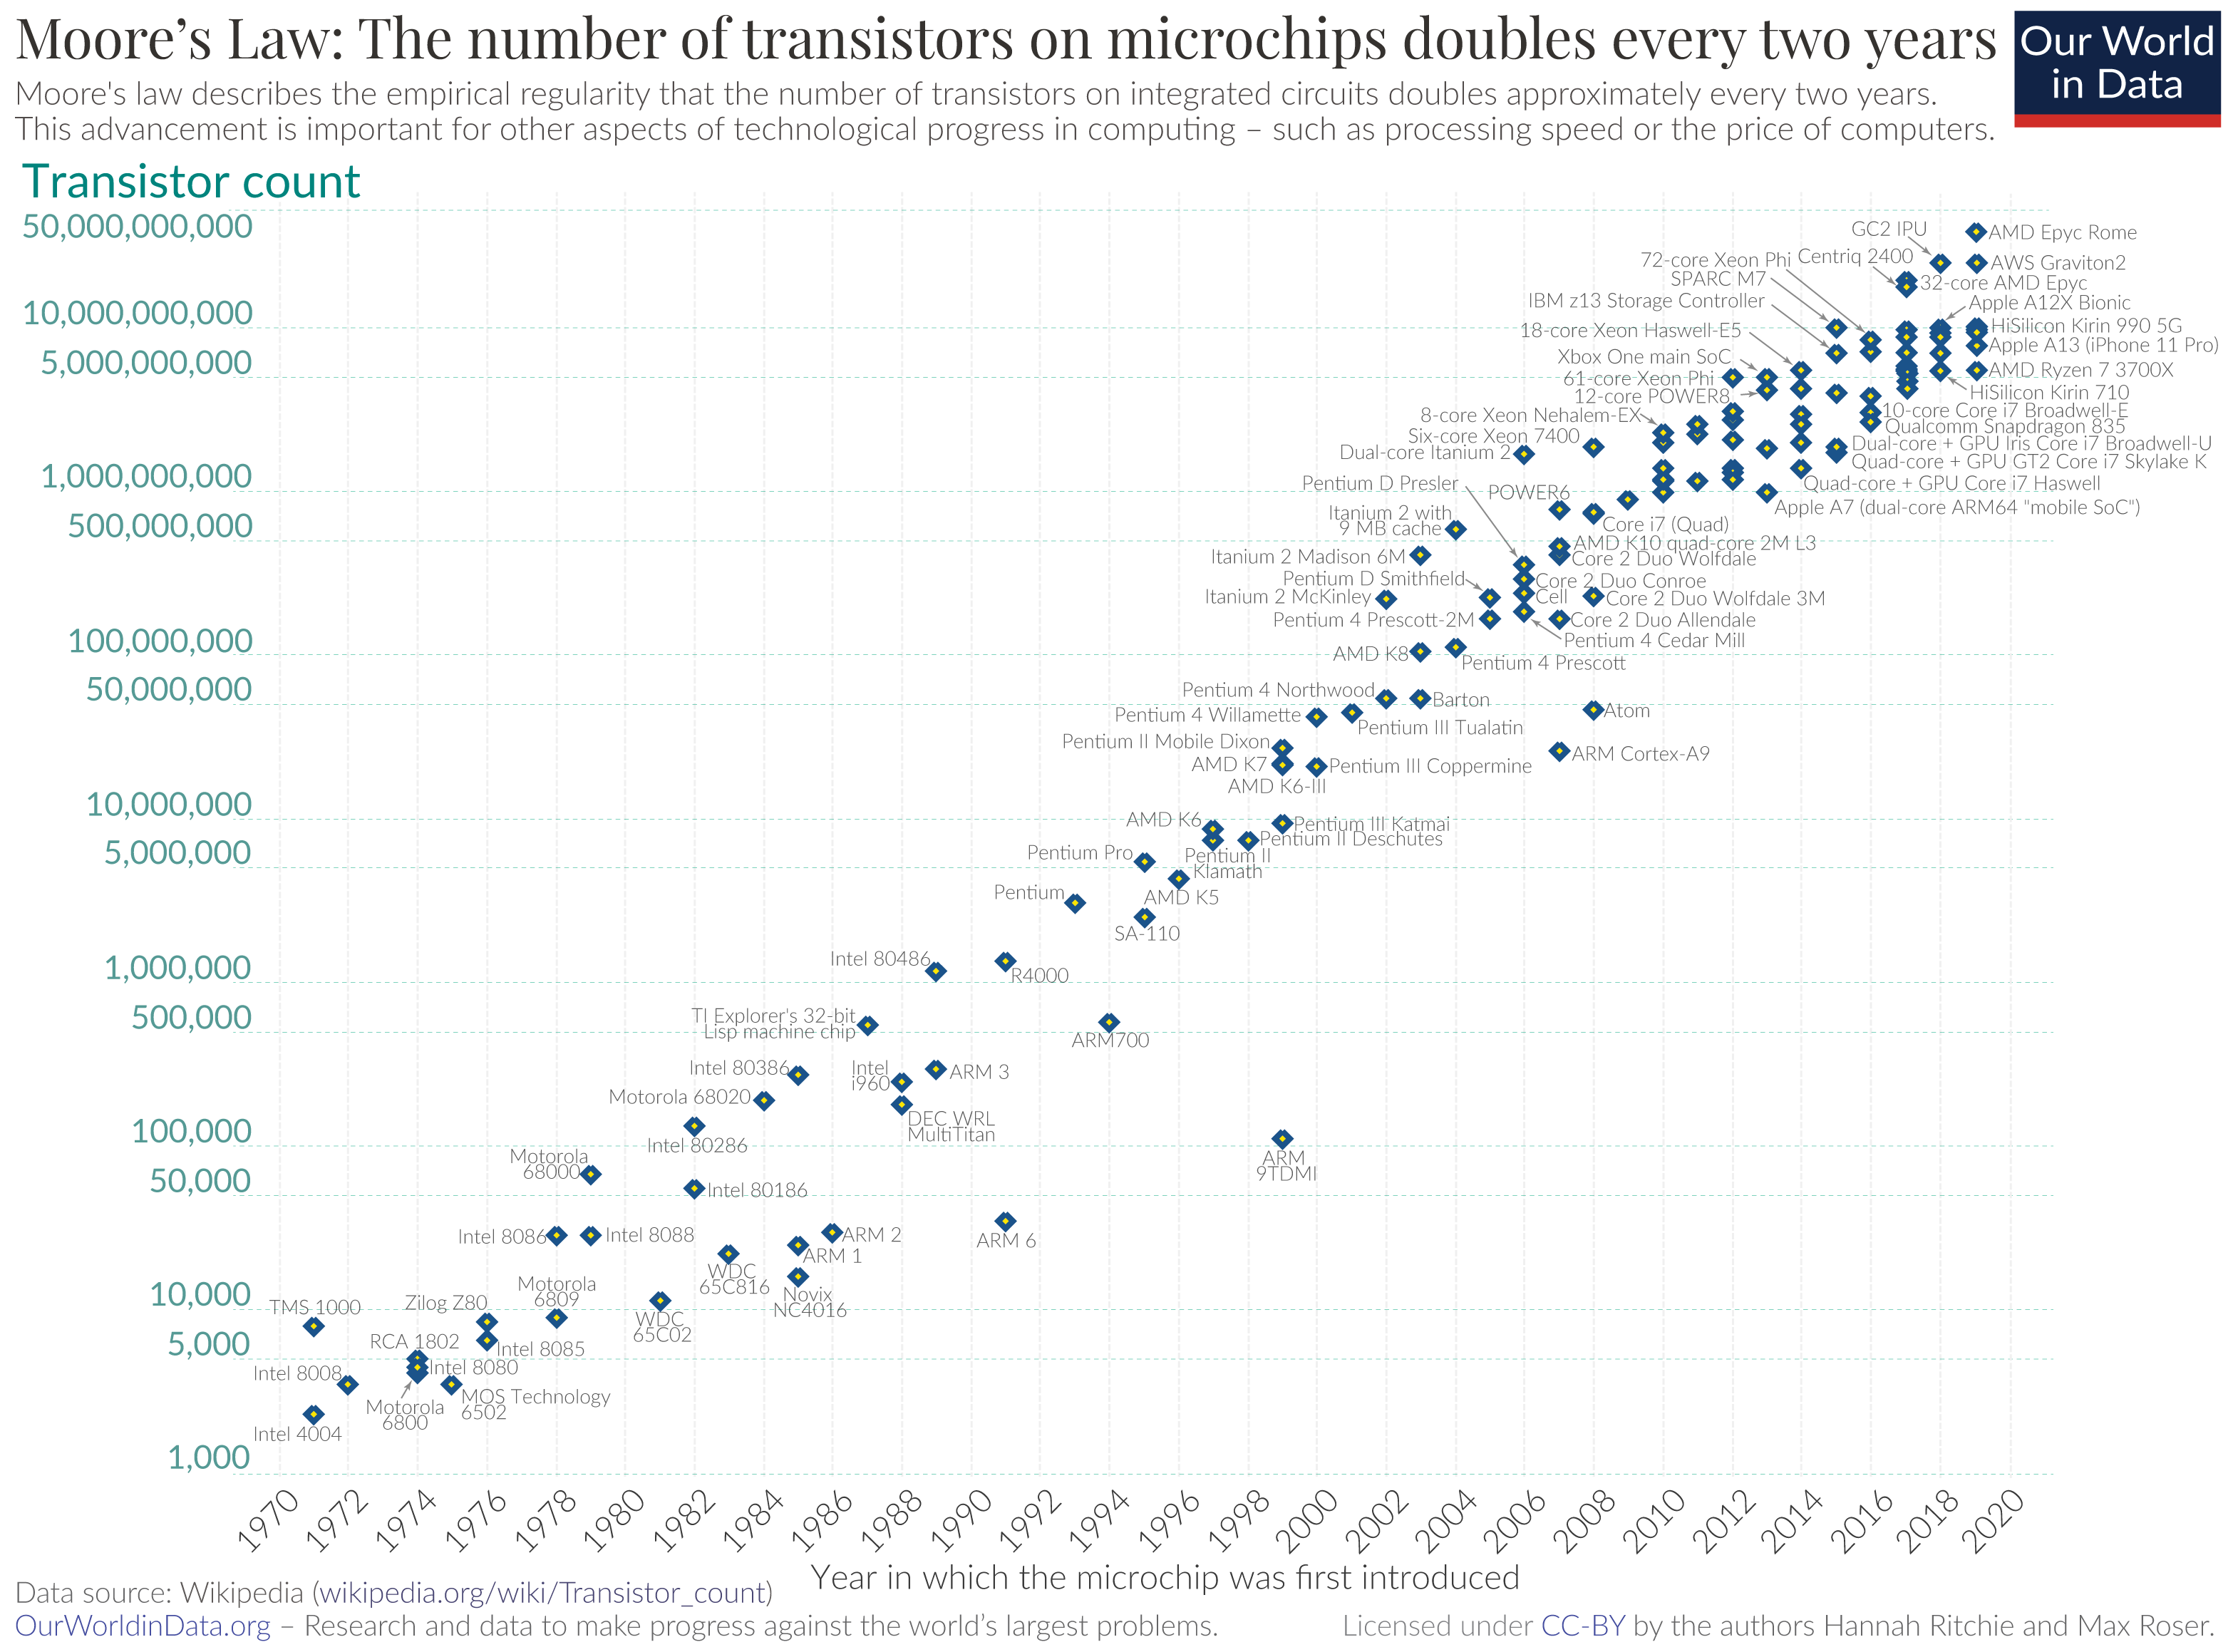
\includegraphics[width=.95 \textwidth]{./images_moores/Moores_Law_Transistor_Count.png}
    \centering
    \caption{Visualization of the fulfillment of Moore's law using a plot of transistor count versus year that microchip was first introduced \cite{owid2020technologicalprogress}.}
    \label{Moores_Law_Transistor_Count}
\end{figure}

 
%Seeing that Moore's Law is not a physical law and is instead a phenomenon arising from social and economic progress, an in-depth explanation of this is warranted.
As Moore first predicted, manufacturers were steadily able to cram more and more components on a single silicone chip. Known as Moore's Law 1.0, manufacturers began to make chips more powerful at the same price every couple of years. Although Moore's Law 1.0 still governs high-end chips (for example, Graphical Processing Units (GPUs), High-end Field Programmable Gate Arrays (FPGAs) and supercomputers), this computing power is too strong for most commercial applications. Instead, we have the variation Moore's Law 2.0 where manufactures deliver a similar level of computing power at a lower price in each successive generation \cite{peper2017end}.

Over this time, the global information technology industry has grown to be a \$5 trillion industry \cite{comptia2021ITindustry}. This doubling of performance and functionality of digital electronics every two years at the same cost is something that our innovation-driven economy has come to rely on. Moore's has held thus far but recent reports show that the the technological drivers underpinning Moore's law are already failing and likely to plateau by 2025 \cite{IEEE2017postmoore}. Although skepticism towards Moore's Law is nothing new\footnote{Skepticism towards Moore's Law has been so prevalent, there's even a joke about it: ``There's a law about Moore's law. The number of people predicting the death of Moore's Law doubles every two years" \cite{economist2016aftermoores}.}, there has been a surge of mutterings amongst the industry especially as components are approaching a fundamental limit of smallness---the atom---and there are slower increases in revenue in conjunction with larger increases in cost \cite{economist2016aftermoores}. In order to continue this ``progress" of computing in a Post-Moore Era, researchers will need to do a comprehensive rethinking of technologies: innovative materials, devices, circuits, system architectures, programming systems, system software and applications \cite{IEEE2017postmoore}. 


Although the history of Moore's Law and the internet and communication technology (ICT) industry\footnote{Internet and communication technology (ICT) are the devices, networking components, applications and systems that combine to allow people and organisations to interact in the digital world. The list of ICT components is continually growing but it can be broadly categorized into hardware, software, transactions, communication technology, data, internet access and cloud computing \cite{techtarget2020ICT}.}
is often recalled as one of innovation and the limitless of human ingenuity, there is another tangible limit that is often overlooked: the carrying capacity of our biosphere for ICT. But before we can explore this limit, let us take a walk through history and see how our earlier limits shaped the current ICT landscape.


%%%%%%%%%%%%%%%%%%%%%%%%%%%%%%%%%%%%%%%%%%%%%%%%%%%%%%%%%%%%%%%%%%%%%%%%
%%%%%%%%%%%%%%%%%%%%%%%%%%%%%%% Limits %%%%%%%%%%%%%%%%%%%%%%%%%%%%%%%%%
\cleardoublepage
\subsection{Human Ingenuity}
 \begin{fquote}[Ronald Reagan][Commencement address at the University of South Carolina, 20 September 1983 \cite{science2004reaganonscience}] 
 There are no such things as limits to growth, because there are no limits on the human capacity for intelligence, imagination, and wonder.
 \end{fquote}
%%%%%%%%%%%%%%%%% Limit #1: Complex Supply Chains  %%%%%%%%%%%%%%%%%%%%%
\subsubsection{The First Limit: Complex Supply \& Production Chains}
Following Moore's first prediction in 1965, the number of transistors on a microchip steadily doubled. But as time went on, the chip-making process became more and more complex with hundreds of stages and a multitude of raw mineral suppliers. 
%This meant you now required a network of materials-suppliers and apparatus-makers to deliver the right upgrade at the right time, otherwise the whole chain would have to grind to a halt. 
There was also minimal visibility along the supply chain: a link on the supply chain typically had no knowledge of the resource limits in another part of the supply chain. Without an understanding of the context where other suppliers were operating, there wasn't a way to know the variability of the supply, quality or quantity of the supply chain. And so if there was a single mineral or component missing from the microchip, the whole chain would have to grind to a halt. In 1991 the United States of America (USA) semi-conductor industry devised its first road map, known as the National Technology Roadmap for Semiconductors. This collaborative effort saw hundreds of engineers from various companies working together to provide this much needed coordination. In 1998 this mapping effort became the International Technology Roadmap for Semiconductors (ITRS) with industry participation also coming from Europe, Japan, Taiwan and South Korea. This type of coordination, where manufactures and suppliers all gather to determine the role they will play, has not been seen in another industry. But its impact was unmistakable: it converted Moore's law from an empirical observation into a self-fullfulling prophecy. New chips followed the law not by chance; they followed Moore's Law because the industry ensured they would \cite{waldrop2016chips, schaller1997moore}.

Although the ITRS was successful at keeping the semi-conductor industry on track with Moore's,there are many modern day risks facing the ICT supply chain. With the onset of the global COVID-19 pandemic, there has been significant disruptions along the upstream part of the supply chain. Lockdowns have forced many component and assembly plants to close. This coupled with suppliers typically operating with very thin inventory levels and travel restrictions have caused delivery delays of essential components \cite{flaviano2021global}. As well, many minerals essential for ICT are critical or conflict minerals (Section \ref{SECTION_CONFLICT_MINERALS}), with a high risk associated with their supply. The potential for geopolitical and economic disruptions to these reservoirs is non-trivial and will be explored later in more detail.


%%%%%%%%%%%%%%%%%%%%%%%%% Limit #2: Heat  %%%%%%%%%%%%%%%%%%%%%%%%%%%%%%
\subsubsection{The Second Limit: Heat}
The first few decades following the wake of Moore's Law saw a substantial increase in clock rates that would have been impossible with just semiconductor scaling alone. During this era, a programmer could simply write sequential code that principally executed in a single thread of control and still dramatically improve performance due to the higher clock rates. But around the mid 2000s high clock frequencies hit their upper limit as we ran into the power limit a chip is able to dissipate. Too hot to continue, clock rates had to be capped and researchers could no longer improve performance with the sequential programming model. But the market and Moore's Law demanded ever-increasing performance. So the microprocessor industry ingeniously innovated and adopted a radical new approach: parallelism. By shifting from a single power-efficient processor (or core) to multiple power-efficient processors on a single chip, we could continue to expand computing capability. Although parallelism is a natural solution from a hardware perspective, it required a complete reinvention of the software and hardware stack \cite{asanovic2009view, pankratius2010guest}.

%%%%%%%%%%%%%%%%%%%%% Limit #3: A Single CPU  %%%%%%%%%%%%%%%%%%%%%%%%%%
\subsubsection{The Third Limit: Computing Power of a Single CPU}
Thanks to parallelism successfully addressing the heat dissipation issue, the ICT industry was able to churn out devices with ever-increasing performance. But again another limit to our growth appeared—there is only so much a single system can scale up. There are physical limits to the die size and continued cramming of components will cause the cost to go up \cite{krzyzanowski2020distributedsystems}. Take the Intel Xeon W-3175X Processor: at 28 cores and 8 billion transistors, this single chip sells for around \$3,000 USD \cite{intel2021processor}. However, in the early 2020s researchers were facing another limit with regards to shrinking circuits: continued scaling with silicon was no longer possible since chips were getting so small they would start experiencing quantum effects. In response to this, researchers are investigating quantum computing and neuromorphic computing. Although the theory is still far ahead of the hardware, the first quantum computers are coming out \cite{newscientist2020IBMquantum, chen2021integrated} and they would theoretically provide a rapid speedup for a limited set of tasks. Other avenues that researchers are investigating are new architectural approaches (including a 3-dimensional skyscrapper versus the current flat 2-dimensional circuit) and finding a substitute material for silicon (one that is just as fast but generates less heat). Only time will tell whether these new research paths come to fruition. But if they did, this technology might be financially inaccessible to the average person. One lead researcher put it best: ``My bet is that we run out of money before we run out of physics" \cite{waldrop2016chips}. From the perspective of Moore's and a single central processing unit (CPU), the limit seems to no longer be a technological one but an economic one.

But society and the ICT industry are still demanding more performance than a single CPU can do, at an even lower cost than last year. To help illustrate this increasing demand and expectations for performance, let us examine Google. When it was founded in 1998, it served 10,000 searches daily; by the end of 2006, it would serve 10,000 searches in a single second. Each Google query requires 1,000 computers to retrieve an answer and is all completed in 0.2 seconds \cite{internetlivestats2021googelsearch}. As of writing in July 2021, there have been 1.6 trillion Google searches so far this year \cite{worldometers2021}.

By unifying advances in computing power with the development of high-speed computer networks, human ingenuity innovated again: distributed systems. Although a distributed system appears as a single coherent system to its users, it is actually a collection of autonomous computing elements (typically geographically dispersed) that communicate and coordinate their actions \cite{van2017distributed}. If you are like me, however, then you do not want to buy multiple computers (and set them up to talk to each other) in order to enjoy enhanced performance. Rather, we would prefer the convenience and elegance of using a single small device that interacts with a single interface that does the computing for us, preferably somewhere invisible to us. And so to continue the steady march of progress, we ushered in the new era of cloud computing. Here, ICT infrastructure is now a utility: you can plug into the infrastructure on-demand, via the internet, to access computing resources—applications, servers (physical and virtual servers), data storage, development tools, networking capabilities—which are hosted at a remote data server managed by a cloud services provider \cite{ibm2020cloudcomputing}. Rather than the average consumer purchasing the latest CPU for a few thousand dollars, technology companies buy in bulk the latest, most powerful microprocessors (that do follow Moore's Law) to power their ``cloud" of server farms\footnote{If you truly wanted to bring the Google experience to your home, Google data centers are now using the AMD second-generation EPYC processor. Featuring 64-cores and a 128-thread 7742 chip, it starts at just \$6,950 USD \cite{techcrunch2019EPYCprocessor}. Just don't forget a single Google query uses approximately 1,000 computers. Best of luck with that endeavour.} \cite{waldrop2016chips}. By sharing these computing resources between customers all over the globe, this new economic model allows consumers to access faster computing for even less money than last year, thereby perpetuating Moore's techno-economic model.


%%%%%%%%%%%%% Limit #4: Biosphere Carrying Capacity  %%%%%%%%%%%%%%%%%%%
\subsubsection{The Fourth Limit? The Biosphere's Carrying Capacity for ICT}
Contrary to what the name suggests, the cloud is a physical entity---it is on the bottom of the sea floor, going through deep sea trenches and reefs to connect us to the internet \cite{starosielski2012warning, blum2012tubes}. Since the late 1970s,  we have laid more than 4 billion kilometers of silica fibers across the world (the distance from Earth to Neptune) \cite{doi:10.1021/cen-09810-cover}. The cloud also lives in the data centers that store, manage and transfer digital information (the data for every photo, video, like, post, search query, or transaction must be stored). These data centres typically are massive air-conditioned warehouses full of computer servers. As an example, Google recently struck a deal with the desert region of Mesa, Arizona to build a 750,000 square foot data center. Although a drought-prone region with strict water conservation measures, the town has guaranteed Google 1 million gallons of water a day to cool their data centre (and up to 4 million if it hits project milestones) \cite{time2020googledatacenterwater}. Unfortunately this water will be ``mined": groundwater bodies (deep aquifers) of water are non-renewable as their rate of recharge is negligible on a human time scale \cite{un2003fao}. Although the cloud has become an integral part of everyday business and life, there is a very real cost to these physical entities. 

Living on a finite planet with a finite amount of resources that can only regenerate so fast, it is becoming increasingly difficult to acquire the raw materials that constitute our devices and cloud infrastructure: the environmental impacts of mining, declining ore grades and the socio-political conflicts surrounding scarce metals, critical metals and conflict minerals (Section \ref{SECTION_ACQUISITION_RAW_MATERIALS}). Despite a growing trend towards recycling ICT devices to recover some of these elements, we still face many challenges including low recycling rates, processing hazardous wastes and waste colonialism (Section \ref{SECTION_END_OF_LIFE_EMISSIONS}).
Although they may be micro, to produce a single 2-gram 32MB DRAM chip requires approximately 1,600g of fossil fuels, 72g of chemical inputs and 32,000g (32L) of water (Section \ref{SECTION_PRODUCTION}). And these are just the potential limit points if we never use our devices. Despite the energy consumption for our personal devices stabilizing (and is even projected to decline) \cite{andrae2015global}, they have instead shifted to our massive cloud infrastructure. In just 2019, Google used 12.4 terrawatt-hours\footnote{12.4 terrawatt-hours is equivalent to 44,640,000,000,000,000 joules} of electricity; if Google were an independent nation, its electricity usage would rank in the top 90 countries worldwide. Just lagging behind Moore's, Google's electricity consumption is also exponentially growing with a doubling rate of every three years \cite{forbes2020googleenergy}. This energy consumption of our devices and cloud infrastructure will be explored further in Section \ref{SECTION_ENERGY_CONSUMPTION}.

Another side of Moore's Law that is often overlooked is how this perpetual demand for better technology also renders older technology obsolete far before their theoretical lifespan. Known as planned obsolescence within the industry, we will explore this flipside to Moore's in greater detail in Section \ref{SECTION_PLANNED_OBSOLESCENCE} to understand how this economic model is pushing our limited resources even closer to our Earth's carrying capacity.

Now that we have examined the history of Moore's and the technological limits it has overcome, let us explore the consequences of this exponential growth on our biosphere and whether the next limit may be a biophysical resource constraint, rather than technological or economical.

%%%%%%%%%%%%%%%%%%%%%%%% Ecology Background %%%%%%%%%%%%%%%%%%%%%%%%%%%%
\subsection{Exponential Growth}
 \begin{fquote}[Donella H. Meadows][Thinking in Systems: A Primer \cite{meadows2008thinking}] 
 There always will be limits to growth. They can be self-imposed. If they aren’t, they will be system-imposed.
 \end{fquote}
 
Although often overlooked in the field of computer science, one of the first lessons you learn as an ecologist is that a finite planet with a finite amount of resources can only support a limited number of organisms. Known as the \textbf{carrying capacity}, this is the maximum sustainable number of individuals per unit area given the finite resources (food, shelter, nutrients, water, space and mates) and conditions (temperature, seasonality, non-nutrient chemicals like pH and salinity, predation-/pathogen-/competitor-pressure and disturbances) present. If these needs are not met, the population will decrease until the resource rebounds. Conversely, a population may overshoot its carrying capacity temporarily but it will stop either abruptly or gradually. In the case of a sudden halt, a population may be stopped at any density; the population tends to grow exponentially until an outside force is exerted, causing the population level to crash. In contrast, a gradually halted constraint is a density-dependent regulation of growth: the population tends to grow exponentially and then slows once it reaches a certain density \cite{waynegoodey2014biology230}. This is also known as a \textbf{logistic} or sigmoid growth, due to its `S' curve shape (Figure \ref{population_logistic_curve}). For those interested in the mathematics behind population growth, please see Appendix \ref{SECTION_APPENDIX_POPULATION_ECOLOGY} for the formulae. 

\begin{figure}[h]
    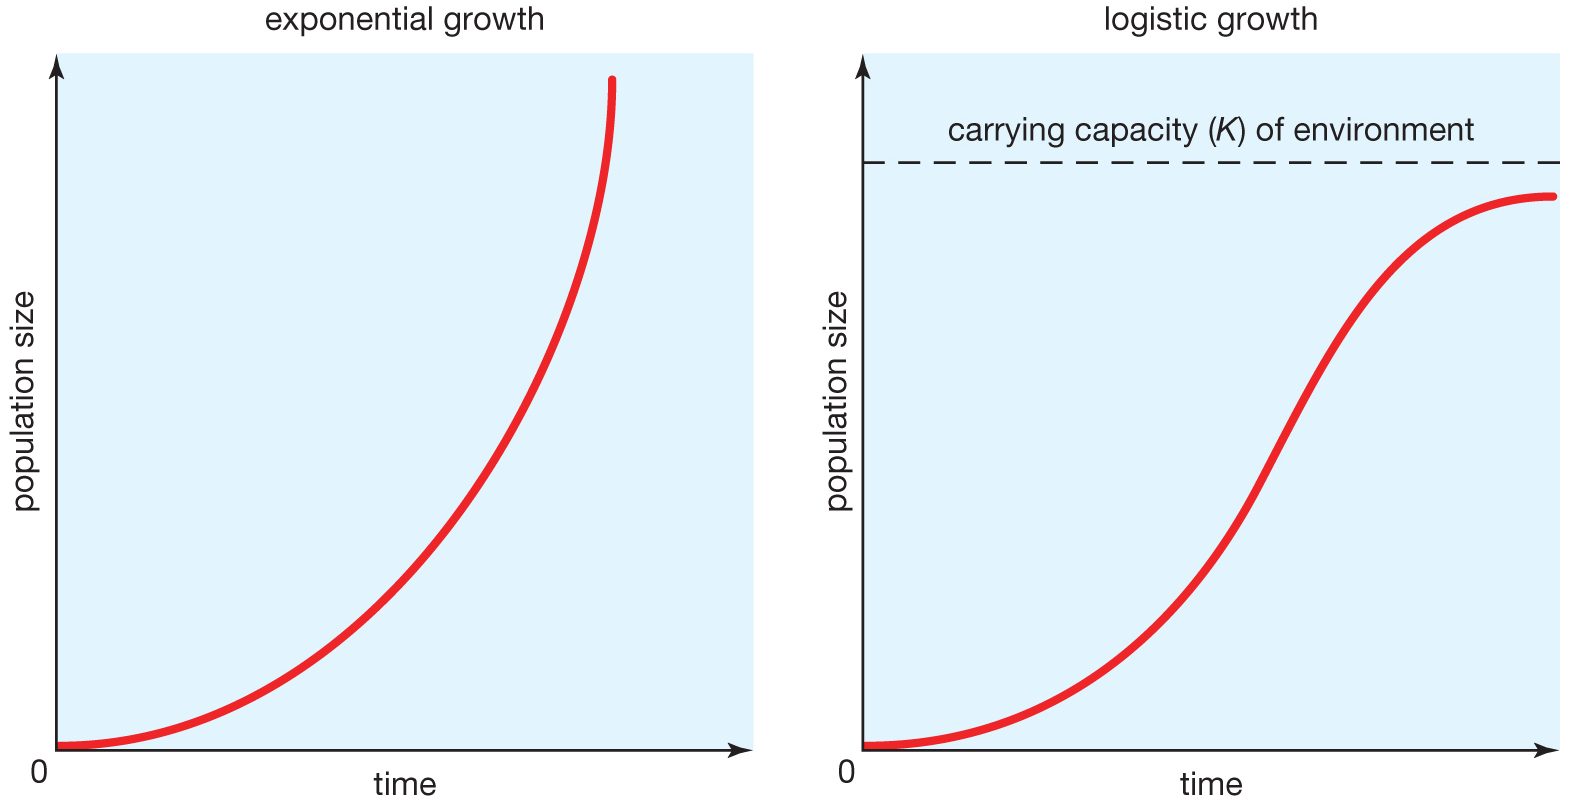
\includegraphics[width=.8 \textwidth]{./images_moores/population_logistic_curve.jpeg}
    \centering
    \caption{Visualization of a population experiencing exponential or logistic growth \cite{britanica2012populationgrowth}.}
    \label{population_logistic_curve}
\end{figure}

This `S' curve, however, is highly idealized. Most populations do not smoothly approach their carrying capacity; they tend to overshoot and crash, then continue to oscillate above and below their carrying capacity, typically settling at just below the carrying capacity (Figure \ref{population_carrying_capacity_oscillate}, green line). Sometimes this exponential growth causes an overshoot resulting in a permanent collapse (Figure \ref{population_carrying_capacity_oscillate}, red line).

\begin{figure}[h]
    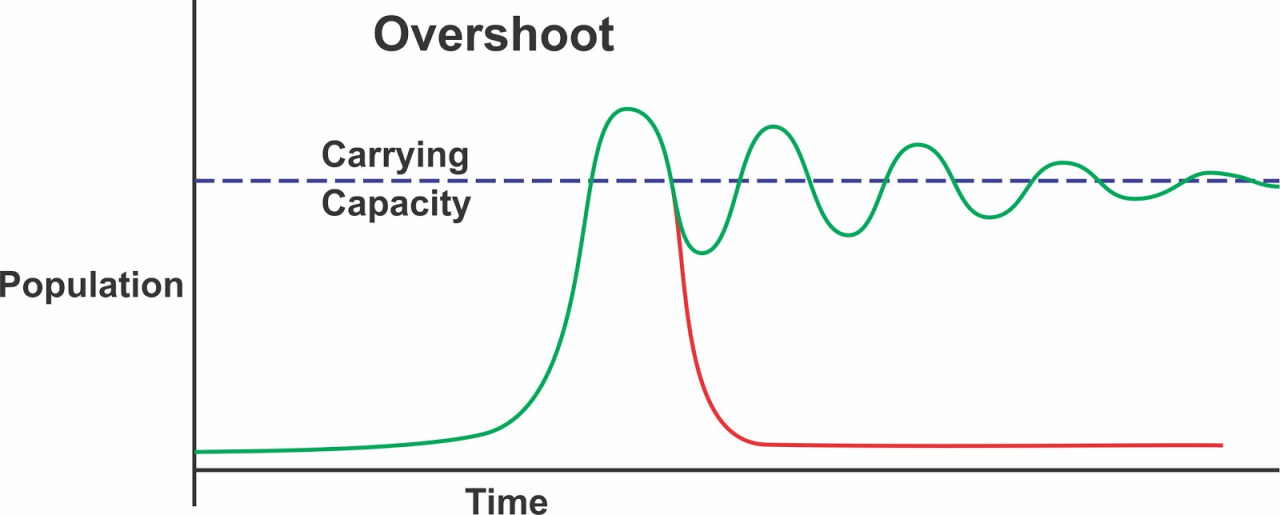
\includegraphics[width=.8 \textwidth]{./images_moores/population_carrying_capacity_oscillate.jpeg}
    \centering
    \caption{Visualization of a population overshoot with constant carrying capacity. In this case, we have a population overshooting its carrying capacity, followed by a crash and either \textbf{(green line)} damped oscillations around its carrying capacity or \textbf{(red line)} a rapid and sudden population collapse \cite{mills2018bumpyroaddown}.}
    \label{population_carrying_capacity_oscillate}
\end{figure}

A common misconception is that a population's carrying capacity $K$ is constant. With the exception of the very short term, the carrying capacity is often fluctuating due to diseases and disturbances. As well, populations may change their own $K$-values. In the case of the human population, the agricultural revolution greatly increased our carrying capacity. Our surrounding ecosystem may also shift our $K$-value; this could be due to a change in conditions (for example, climate change and ocean acidification) or a superior competitor is introduced (perhaps a new invasive species or a new technology emerges that greatly consumes the rare earth elements essential for our ICT devices). Although a species may be able to temporarily overshoots its environment's carrying capacity, in doing so the species degrades its environment and therefore reduces the carrying capacity. And so the population graph looks more like Figure \ref{population_carrying_capacity_declining} where we have an overshoot that is still oscillating but is also steadily declining along with its declining carrying capacity \footnote{There are many other population dynamics outside the scope of this paper (including the fascinating continual oscillation of predator and prey populations). If interested, I would strongly recommend the introductory Ecology textbook by Cain et al. \cite{cain2011ecology}.}. A classic example of this is the human population's prolonged exceeding of its carrying capacity. In doing so, we have also eroded the Earth's \textbf{ecosystem services} (moderation of weather extremes, mitigation of droughts and floods, nutrient cycling, reduced erosion along shorelines, maintenance of biodiversity, purification of air and water, generation and preservation of soils and soil fertility, pollination, dispersal of seeds, protection from solar ultraviolet radiation, aesthetic beauty and recreation, et cetera), thus reducing its capacity to support us.

\begin{figure}[h]
    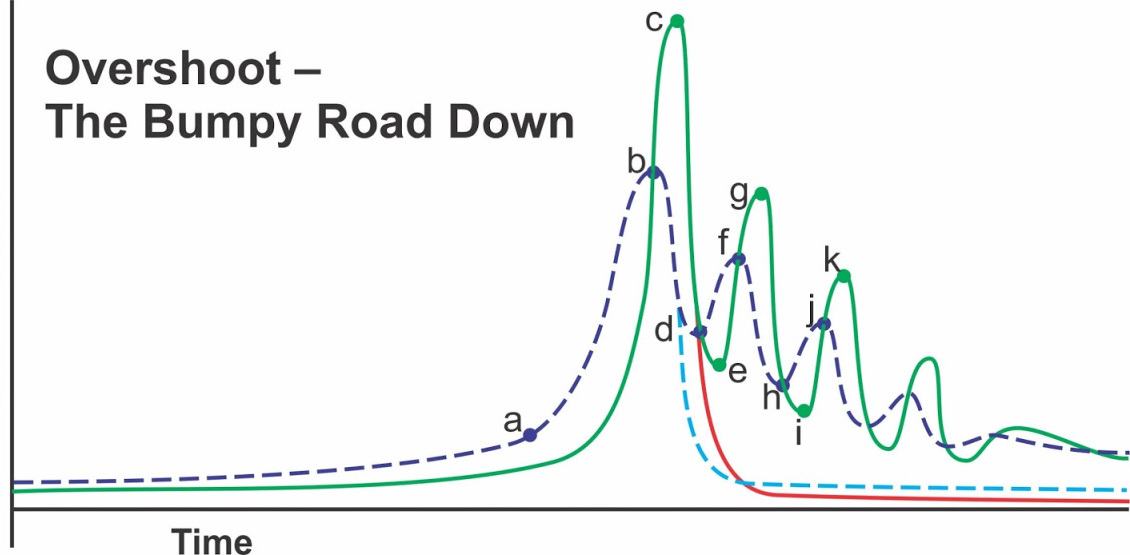
\includegraphics[width=.8 \textwidth]{./images_moores/population_carrying_capacity_declining.jpeg}
    \centering
    \caption{Visualization of a population overshoot (green) with declining carrying capacity (blue). The light blue and red lines also represent the alternative situation where the overshoot results in a fast and permanent crash of the carrying capacity and population \cite{mills2018bumpyroaddown}.}
    \label{population_carrying_capacity_declining}
\end{figure}

% So why don't populations expand infinitely? While a very complex answer with many limits to growth, they can be broadly classified into three categories: 
% \begin{itemize}
%     \item \textbf{Intraspecific Competition} (within-species): a population uses up its own resources. For example, there may be a limited number of available mates, prey or water.
%     \item \textbf{Interspecific Competition} (among-species): a population runs out of resources because another population has used them up.
%     \item \textbf{Disturbance}: a population is stopped by a disturbance before it runs short of resources. This is a very diverse category that involves anything non-competitive, including seasons (winter, dry season, etc.), predation and catastrophe (fire, wind, landslide, earthquake, etc.). 
% \end{itemize}

By analogy with the ecological notion of carrying capacity, there are biophysical limits that constrain the number of ICT devices that the Earth can sustainably support. These limits are not just resource constraints (limits to stocks) but also the rate at which we can replenish resources (limits to flows). Using the COVID-19 pandemic as an example, this limit to flows was apparent with the shortage of personal protective equipment (PPE) and toilet paper; for climate change, we could transition all of our economies to clean energy but the rate we do so might not be fast enough. %This type of research belongs to the field of life cycle assessment resource depletion and is strongly encouraged for further readings.
These biophysical limits---including resource constraints, limits to flows, assimilative capacity, nutrient cycling and wastes--- with respect to Moore's will be explored in more detail in the upcoming sections.

Despite these limits to growth, we have seen a plethora of exponentials within the Anthropocene\footnote{The \textbf{Anthrorpocene} is the unofficial global geological epoch that the Earth has moved into (from the previous Holocene epoch which began approximately 11,650 years ago at the end of the Last Glacial Maximum), which is characterized by human activity becoming a global geological force that is changing our climate and ecosystems. Much debate still exists as to whether it should be declared a new epoch (and if so, should it be at the start of the Industrial Revolution in the 1800s, the first atomic bomb testing in 1945 or the Great Acceleration in 1950); the main criteria for epochs is whether humans have changed the Earth system enough that it shows up in the fossil records \cite{nationalgeographic2019anthropocene, steffen2011anthropocene}.}: human population, CO$_2$ concentration, total real GDP, international tourism, damming of rivers \cite{steffen2011anthropocene}, big data \cite{statista2021bigdata}, mining production \cite{mudd2007sustainability}, memory capacity, processing speed \cite{owid2020technologicalprogress} and of course, Moore's Law. 
Although the folklore of infinite human ingenuity has been repeated time and time again, there are limits due to the creation, implementation and delivery of ingenuity. This gives rise to the \textbf{ingenuity gap}: as our world becomes more complex with new technology, the ingenuity required to solve our new problems is rapidly becoming outpaced by the supply of ingenuity required to solve it \cite{homer2001ingenuity}. In addition to this gap between theoretical infinite ingenuity and the actual application of ingenuity to our problems, we must also reckon with the biophysical laws that govern our planet. It would be a lovely continuation of the Moore's legend if human ingenuity could innovate our way out of this biophysical resource limit. But due to the nature of exponential growth, the ingenuity gap and the underlying systematic issues underpinning the ICT industry, it seems unlikely. So the question becomes less of \textit{if} these exponentials will stop, but a question of \textit{how, when} and \textit{whether} the inevitable overshoot crash will be followed by dampening oscillations or a fast and permanent crash.

%%%%%%%%%%%%%%%%%%%%%%%%%%%%%%%%%%%%%%%%%%%%%%%%%%%%%%%%%%%%%%%%%%%%%%%%
%%%%%%%%%%%%%%%%%%%%%%% Planned Obsolescence  %%%%%%%%%%%%%%%%%%%%%%%%%%
\cleardoublepage
\section{Artificially Shortened Lifespan of ICT Devices} \label{SECTION_PLANNED_OBSOLESCENCE}
 \begin{fquote}[Henry Ford II][1955 \cite{sugrue1995forget}] 
 Obsolescence is the very hallmark of progress.
 \end{fquote}

% Gadget Today, Garbage Tomorrow
Irregardless of how well human ingenuity can manufacture a more efficient or powerful device, a key factor exacerbating our biophysical resource limits is how long we can use an ICT device before it truly is trash. A longer lifespan reduces the total resource consumption for the global ICT sector; a shorter lifespan means more raw materials are required, more devices must be manufactured and more devices must be disposed of or recycled. Unfortunately people often upgrade their ICT devices before the end of the lifespan (Figure \ref{estimated_lifespan_ICT}). Despite mobile phones being designed to last at least 7 years, the average American changes their mobile phone every year while the average European does so every 18 months \cite{bournay2006vital, webfx2016lifespanICT}. These ex-marvels of technology are still functioning but are often pre-maturely disposed of or lying around unused. Sometimes the discrepancy between actual versus theoretical lifespan arises from unforeseen circumstances that a company did not anticipate. But more often it is due to a deliberate effort by companies to ``[instill] in the buyer the desire to own something a little newer, a little better, a little sooner than necessary" \cite{stevens1960planned}.

\begin{figure}[h]
    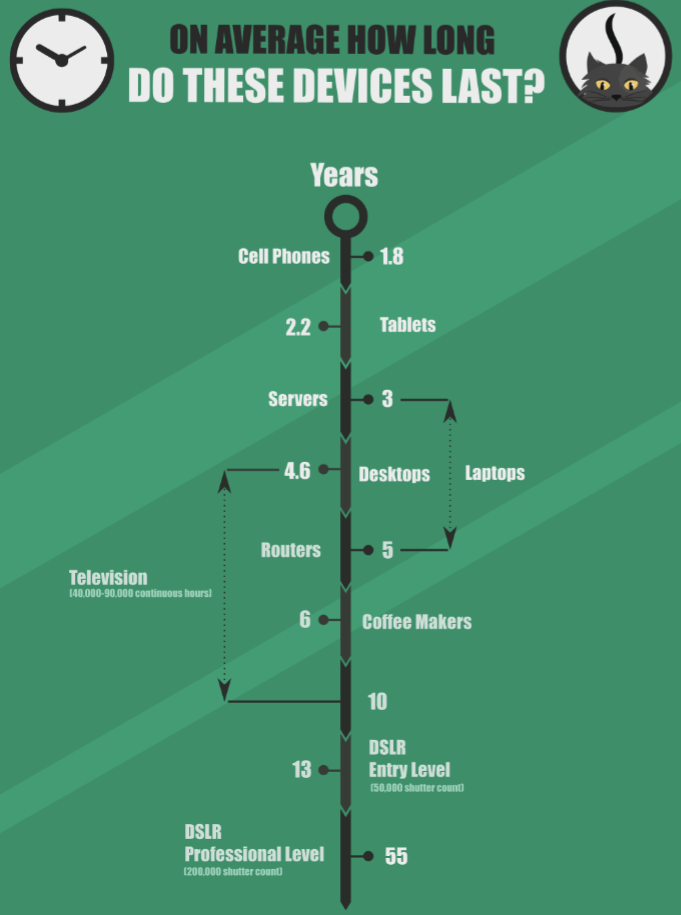
\includegraphics[width=.7 \textwidth]{./images/lifespan_ICT_US.png}
    \centering
    \caption{The estimated 2015 lifespan of common electrical and ICT devices in the United States of America \cite{webfx2016lifespanICT}.}
    \label{estimated_lifespan_ICT}
\end{figure}


%%%%%%%%%%%%%%%%%%%%%%%% Planned Obsolescence %%%%%%%%%%%%%%%%%%%%%%%%%%
\subsection{Planned Obsolescence} \label{SECTION_PLANNED_OBSOLESCCENCE}

Within our recollection of Moore's history, we predominantly focused on the technological aspect. Although incredibly important, Moore's is not just a technological model---it is also an economic one. In order to bring better technology to market every 2 years, you need to manufacture both the technological capabilities and the consumer desire to discard their old products so they can purchase these new products. Without this reinforcing feedback loop, manufacturers would not be able to finance their extensive research and new fabrication plants required for the technological aspect. By leveraging the principles of \textbf{planned obsolescence}---the production of goods with uneconomically short useful lives so that customers will have to make repeat purchases
\cite{bulow1986economic}---the ICT industry has artificially manufactured a consumer demand to perpetuate the steady march of Moore's.

So how has the ICT industry fabricated this demand? Planned obsolescence is neither a new phenomena nor one only within the high technology industry: firms have an economic incentive to introduce new products that make their old products obsolete in order to stimulate replacement buying by consumers. This can be achieved through a number of \textit{physical obsolescence} mechanisms: limited functional life design (``death dating"), designing for limited repair (lack of affordable repair options or access to replacement parts), and design aesthetics that lead to reduced satisfaction (for example, a pristine and polished initial appearance that with everyday use will quickly become damaged, engendering user dissatisfaction and premature disposal) \cite{guiltinan2009creative}. A classic example of this mechanism is Apple's batteries: they are not removable by a customer and have a purposefully short lifespan. Since the product can only be fixed by Apple, they can charge sufficiently high repair prices so that it makes more sense for a customer to buy a new product instead of replacing the battery \cite{keeble2013culture}.

Even faster replacement can be achieved by fostering \textit{technological obsolescence}. This is achieved by designing a functional enhancement that adds or upgrades product features. Sometimes these are revolutionary (adding a camera feature to a cell phone), but often they are the near constant progression of technology (making new laptops with increased memory or reduced weight) \cite{guiltinan2009creative}. This is a common practice amongst mobile phone companies who typically release a new model or updated model every year. It also coincides with the year or two mobile phone contract (and Moore's), which allows people to get the latest phone on the market. There is a large psychological aspect to this phenomenon, so those interested are recommended to take a deep dive with \cite{keeble2013culture}. 

With \textit{style obsolescence}, a product becomes less fashionable and unwanted when a newer trend comes out. Consumers here are motivated by aesthetic considerations or by the implications in relation to their identity construction. Often the product is functional and working in every way other than aesthetics but since the product is no longer `in style' it will be replaced. Another technique is \textit{postponement obsolescence}. A company has technology that can be added to all of their products, but only adds the best technology to their flagship product while the cheaper models have their second rate technology. Within a few years the flagship models will have even newer technology and so the lower end models will typically have the flagship model's technology from years past \cite{keeble2013culture}.

In contrast, durable goods producers face a challenge in maintaining a high rate of sales growth: the more reliable and long-lasting the product, the longer the repeat purchase cycle and the slower the rate of sales growth. Durability also causes a greater competition between new and used versions. This creates an opportunity for a used market which will cause a decrease in price of the next generation of replacement products \cite{guiltinan2009creative}. Often the cost of product disposal is externalized to the community and is not a real cost to the producer. We could ask firms to voluntarily pay for their disposal or to reduce the rate at which new product improvements are brought to market, but this would be akin to requesting unilateral competitive disarmament \cite{guiltinan2009creative}. The literature on public policy initiatives for planned obsolescence of ICT devices is rather sparse, but we will briefly discuss the growing global movement for citizens to have the right to repair their products. Although not a complete solution to planned obsolescence, it would help empower consumers to extend their device's lifespan.

 %Unfortunately the full cost of resource depletion, environmental and health impacts are often externalized, thereby giving manufacturers the economic incentive to produce non-durable goods and to prematurely obsolete their products.


%%%%%%%%%%%%%%%%%%%%%%% Right to Repair %%%%%%%%%%%%%%%%%%%%%%%%%%%%%%%%
\subsection{The Right To Repair}\label{SECTION_RIGHT_TO_REPAIR}
A straightforward way to extend an ICT device's life is to maintain, repair or refurbish it \cite{zerowastecanada2017hierarchy}. Unfortunately, this is not always an option for consumers. As of 2021 in the European Union, four types of electrical appliances (displays, washing machines, dishwashers and fridges) have to be made more easily repairable and longer-lasting. Although a major step forward, there are still many holes: a limited scope (no smartphones or laptops), restricted access of certain spare parts and repair manuals to professional repairers, a long delivery time of spare parts and no requirement for manufactures to update software throughout the lifetime of a product \cite{EUrighttorepair2021}.

Despite strong support amongst Canadians, a bill that would give consumers the right to repair their ICT devices, appliances and vehicles was voted down in 2019 \cite{CArighttorepair2020fail}. In 2021 a national bill was introduced; it is not a true Right to Repair but instead a first step \cite{CArighttorepair2021national}. Meanwhile in the United States of America (USA), an executive order was signed which encourages the Federal Trade Commission to limit equipment manufacturers from restricting people's ability to use independent repair shops or perform their own repairs. Although this is a significant step forward for the Right to Repair movement, it continues to face strong opposition from many companies, including John Deere (farm and construction equipment), Microsoft and Apple \cite{cbc2021farmersrighttorepair}.

By utilising each of these planned obsolescence techniques, the ICT industry has manufactured an unyielding consumer demand for newer, faster and more powerful technology while purposefully blocking consumers from repairing their devices. Simultaneously, researchers have repeatedly innovated to meet this demand for new technology for over half a century. Although obsoleting our products and technology has led to significant technological progress, raised living standards and increased national wealth, our human ingenuity has also been channeled to sell more products rather than benefiting humanity. Unfortunately, every ICT device produced has left an ecological footprint on this planet by the resources and energy they consume and the wastes they leave behind. Artificially shortening the lifespan of ICT devices has expedited the rate we consume our biosphere's finite set of resources, thereby accelerating the rate our exponential growth will reach our biophysical limits.

%%%%%%%%%%%%%%%%%%%%%%%%%%%%%%%%%%%%%%%%%%%%%%%%%%%%%%%%%%%%%%%%%%%%%%%%
%%%%%%%%%%%%%%%%%%%%%%%%%%% Limits to Growth %%%%%%%%%%%%%%%%%%%%%%%%%%%
%%%%%%%%%%%%%%%%%%%%%%%%%%%%%%%%%%%%%%%%%%%%%%%%%%%%%%%%%%%%%%%%%%%%%%%%
\cleardoublepage
\section{Limits to Moore's Exponential Growth} 
 \begin{fquote}[Donella H. Meadows][Limits to Growth: The 30-Year Update \cite{meadows2004limitsupdate}] 
 The idea that there might be limits to growth is for many people impossible to imagine. Limits are politically unmentionable and economically unthinkable. The culture tends to deny the possibility of limits by placing a profound faith in the powers of technology, the workings of a free market, and the growth of the economy as the solution to all problems, even the problems created by growth.
 \end{fquote}
 
Now that we have a better understanding of exponential growth and the physical limits to it, let us turn our attention back to Moore's. 
%Although interspecific (between) competition and major disturbances are possibilities for the end of Moore's (especially with climate change eroding our ecosystem services), those are often stochastic in nature. Instead I would like to focus on the intraspecific (within) competition of our ICT devices:
Rather than exploring external shocks (for example, a global pandemic or climate change eroding our ecosystem services), we will focus on internal dynamics and competition: in the pursuit of building ICT that are faster and cheaper each year, will we run out of the very resources necessary to sustain this complex supply chain? From the cradle to the grave of each device, we must mine the the raw materials, process and manufacture our devices, distribute them to consumers, use them and then discard them \cite{andrae2015life}. If there is a bottleneck anywhere along this chain, this may be the limit point to the last half century of exponential growth. Rather than exploring the technological limits of Moore's, we will explore in the next few sections the physical constraints, resource constraints and the constraints on the environmental and ecosystem integrity that the Earth imposes on Moore's.
 
 
 %%%%%%%%%%%%%%%%%%%%%%%%%%%%%%%%%%%%%%%%%%%%%%%%%%%%%%%%%%%%%%%%%%%%%%%%
%%%%%%%%%%%%%%%%%%%%%%%%%%% Production  %%%%%%%%%%%%%%%%%%%%%%%%%%%%%%%%
%\cleardoublepage
\subsection{Manufacturing a Chip} \label{SECTION_PRODUCTION}
 \begin{fquote}[Arthur Rock\footnote{Arthur Rock is an American businessman and venture capitalist, investing in such iconic tech companies as Fairchild Semiconductor, Intel, Scientific Data Systems, Teledyne and Apple Computer \cite{hbs2021arthurrock}.}][Moore's Second Law (or Rock's Law) \cite{arthurrock2009rockslaw}]
 The cost of a semiconductor chip fabrication plant doubles every four years.
 \end{fquote}

Although Rock's Law %(sometimes referred as Moore's Second Law) 
has not held, the process to fabricate a chip is still extensive and very costly. Unfortunately, every time the size is halved, manufacturers need a new generation of more precise photolithography machines. These new fabrication lines are typically a multi billion dollar investment, which has forced a massive consolidation in the chip-making industry to be a handful of multinationals \cite{waldrop2016chips}.

So how do we manufacture one of these chips? For the central processing unit (CPU), the semiconductor microchip consists of a highly purified silicone wafer (to be of Electronic Grade Silicon, you may only have 1 alien atom for every billion silicon atoms \cite{intel2011makingachip}). Although this high purity is integral to modern computing efficiency, the production of a silicon wafer uses 160 times the energy required for typical industrial grade silicon \cite{williams20021}. Next comes the fabrication of chips on a silicon wafer that creates a series of patterned layers of various materials. This fabrication stage consists of hundreds of precisely controlled steps, including ion implantation, high-k dielectric deposition, photo lithography, etching, metal deposition and metal layering. Finally, these wafers are tested, sliced into dies and then assembled with a heatspreader (a thermal interface that keeps the processor cool during operation) to form the completed processor \cite{intel2011makingachip}. A diagram of this process is summarized in Figure \ref{production_chip}. To produce a single 2-gram 32MB DRAM chip, the process requires approximately 1,600g of fossil fuels, 72g of chemical inputs and 32,000g (32L) of water. The fossil fuels used in production total 600 times the mass of the final product; in comparison, automobiles and refrigerators have a factor of  1-2 \cite{williams20021}. Although these new methods yield more precise small-scale devices, performing thermal oxidative processes to produce thin layers of oxidized silicone has resulted in a large increase in energy demand to produce semi-conductor chips  \cite{gutowski2009thermodynamic}. Unfortunately, these values are very out of date: the silicon wafer energy and the 2-gram microchip study were conducted in 2002. No newer estimates are available. This lack of data and ICT transparency is a common narrative we will see in the upcoming sections and it makes it very difficult to quantify these biophysical limits.

\begin{figure}[h]
    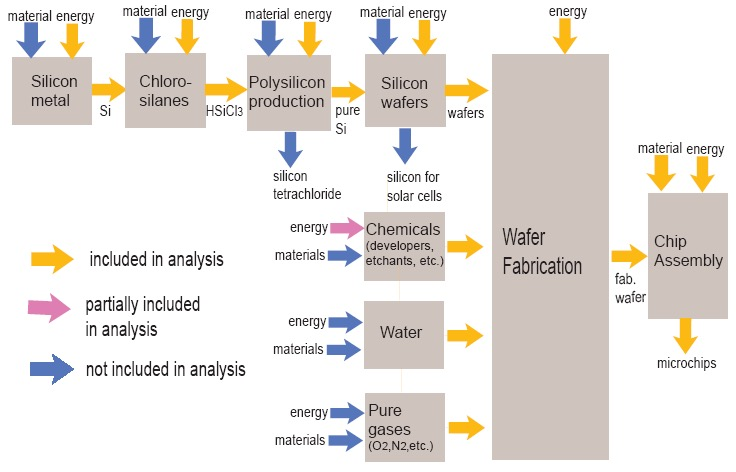
\includegraphics[width=.9 \textwidth]{./images/production_chip.jpg}
    \centering
    \caption{Network of manufacturing processes in chip manufacturing \cite{williams2004environmental}.}
    \label{production_chip}
\end{figure}

In general most emissions associated with an ICT device comes from this production stage, specifically during the manufacturing of the printed circuit board. However, smaller devices, smaller screens and devices with less memory tend to have less embodied greenhouse gas emissions\footnote{Embodied emissions refer to the emissions that occur in the ``upstream" life cycle stage, which correspond to the first two stages of the life cycle analysis: resource extraction and production \cite{teehan2013comparing}.} \cite{louis2020sources, teehan2013comparing}. Overall embodied greenhouse gas emissions for newer products are 50-60\% lower than corresponding older products with similar functionality. This decrease can largely be attributed to a reduction in total mass and a proportional decrease in integrated circuit content \cite{teehan2013comparing}. Although we are producing more efficient devices, Moore's law has meant we are using our devices for far shorter than their theoretical lifespan and our demand for what they can do has also increased. This has resulted in us producing more microchips than necessary and newer ICT technology being far more powerful than its predecessors. And so paradoxically our efficiency gains have created a net increase in embodied greenhouse gas emissions within the ICT product community \cite{ryen2015consumption}.


% The international community takes a production-based approach to measuring a country’s emissions: a country is responsible for the emissions associated with the extraction of raw materials, production of goods and disposal of waste within their borders. This loophole has resulted in yet another game of hot-potato where developed countries export their emissions to developing countries. Although international accounting methodologies is beyond the scope of the paper, the majority of ICT emissions come from its production emissions \cite{hertwich2011greenhouse} and so we thought it pertinent to briefly mention it in Appendix \ref{SECTION_APPENDIX_RESPONSIBILITY_OF_EMISSIONS}.
 
%%%%%%%%%%%%%%%%%%%%%%%%%%%%%%%%%%%%%%%%%%%%%%%%%%%%%%%%%%%%%%%%%%%%%%%%
%%%%%%%%%%%%%%%%%%% Acquisition of Raw Materials  %%%%%%%%%%%%%%%%%%%%%%
\subsection{Mining for Smartphones} \label{SECTION_ACQUISITION_RAW_MATERIALS}
In accordance with Moore's Law, every 18 months we must have more powerful chips; to fulfill this, we must also consume metals and rare earth elements that need to be mined or recycled (Section \ref{SECTION_RECYCLING}). Let us first examine the elements of a smartphone (Figure \ref{ELements_Of_Smartphone}). Although metals comprise approximately 30\% of its mass, less than 1\% of its weight is an assortment of ``spice metals": Tin (1\%), Silver (0.5\%), Gold ($<0.1\%$), Tantalum (trace), Palladium (trace), Indium (trace) and Rare Earth Elements (REE) \cite{bournay2006vital, compoundinterest2014, reller2009mobile}. For a more extensive breakdown of the raw materials and the manufactured parts of a smartphone, please see \cite{andrae2015life} (Table 1 and 2 respectively). 

\begin{figure}[h]
    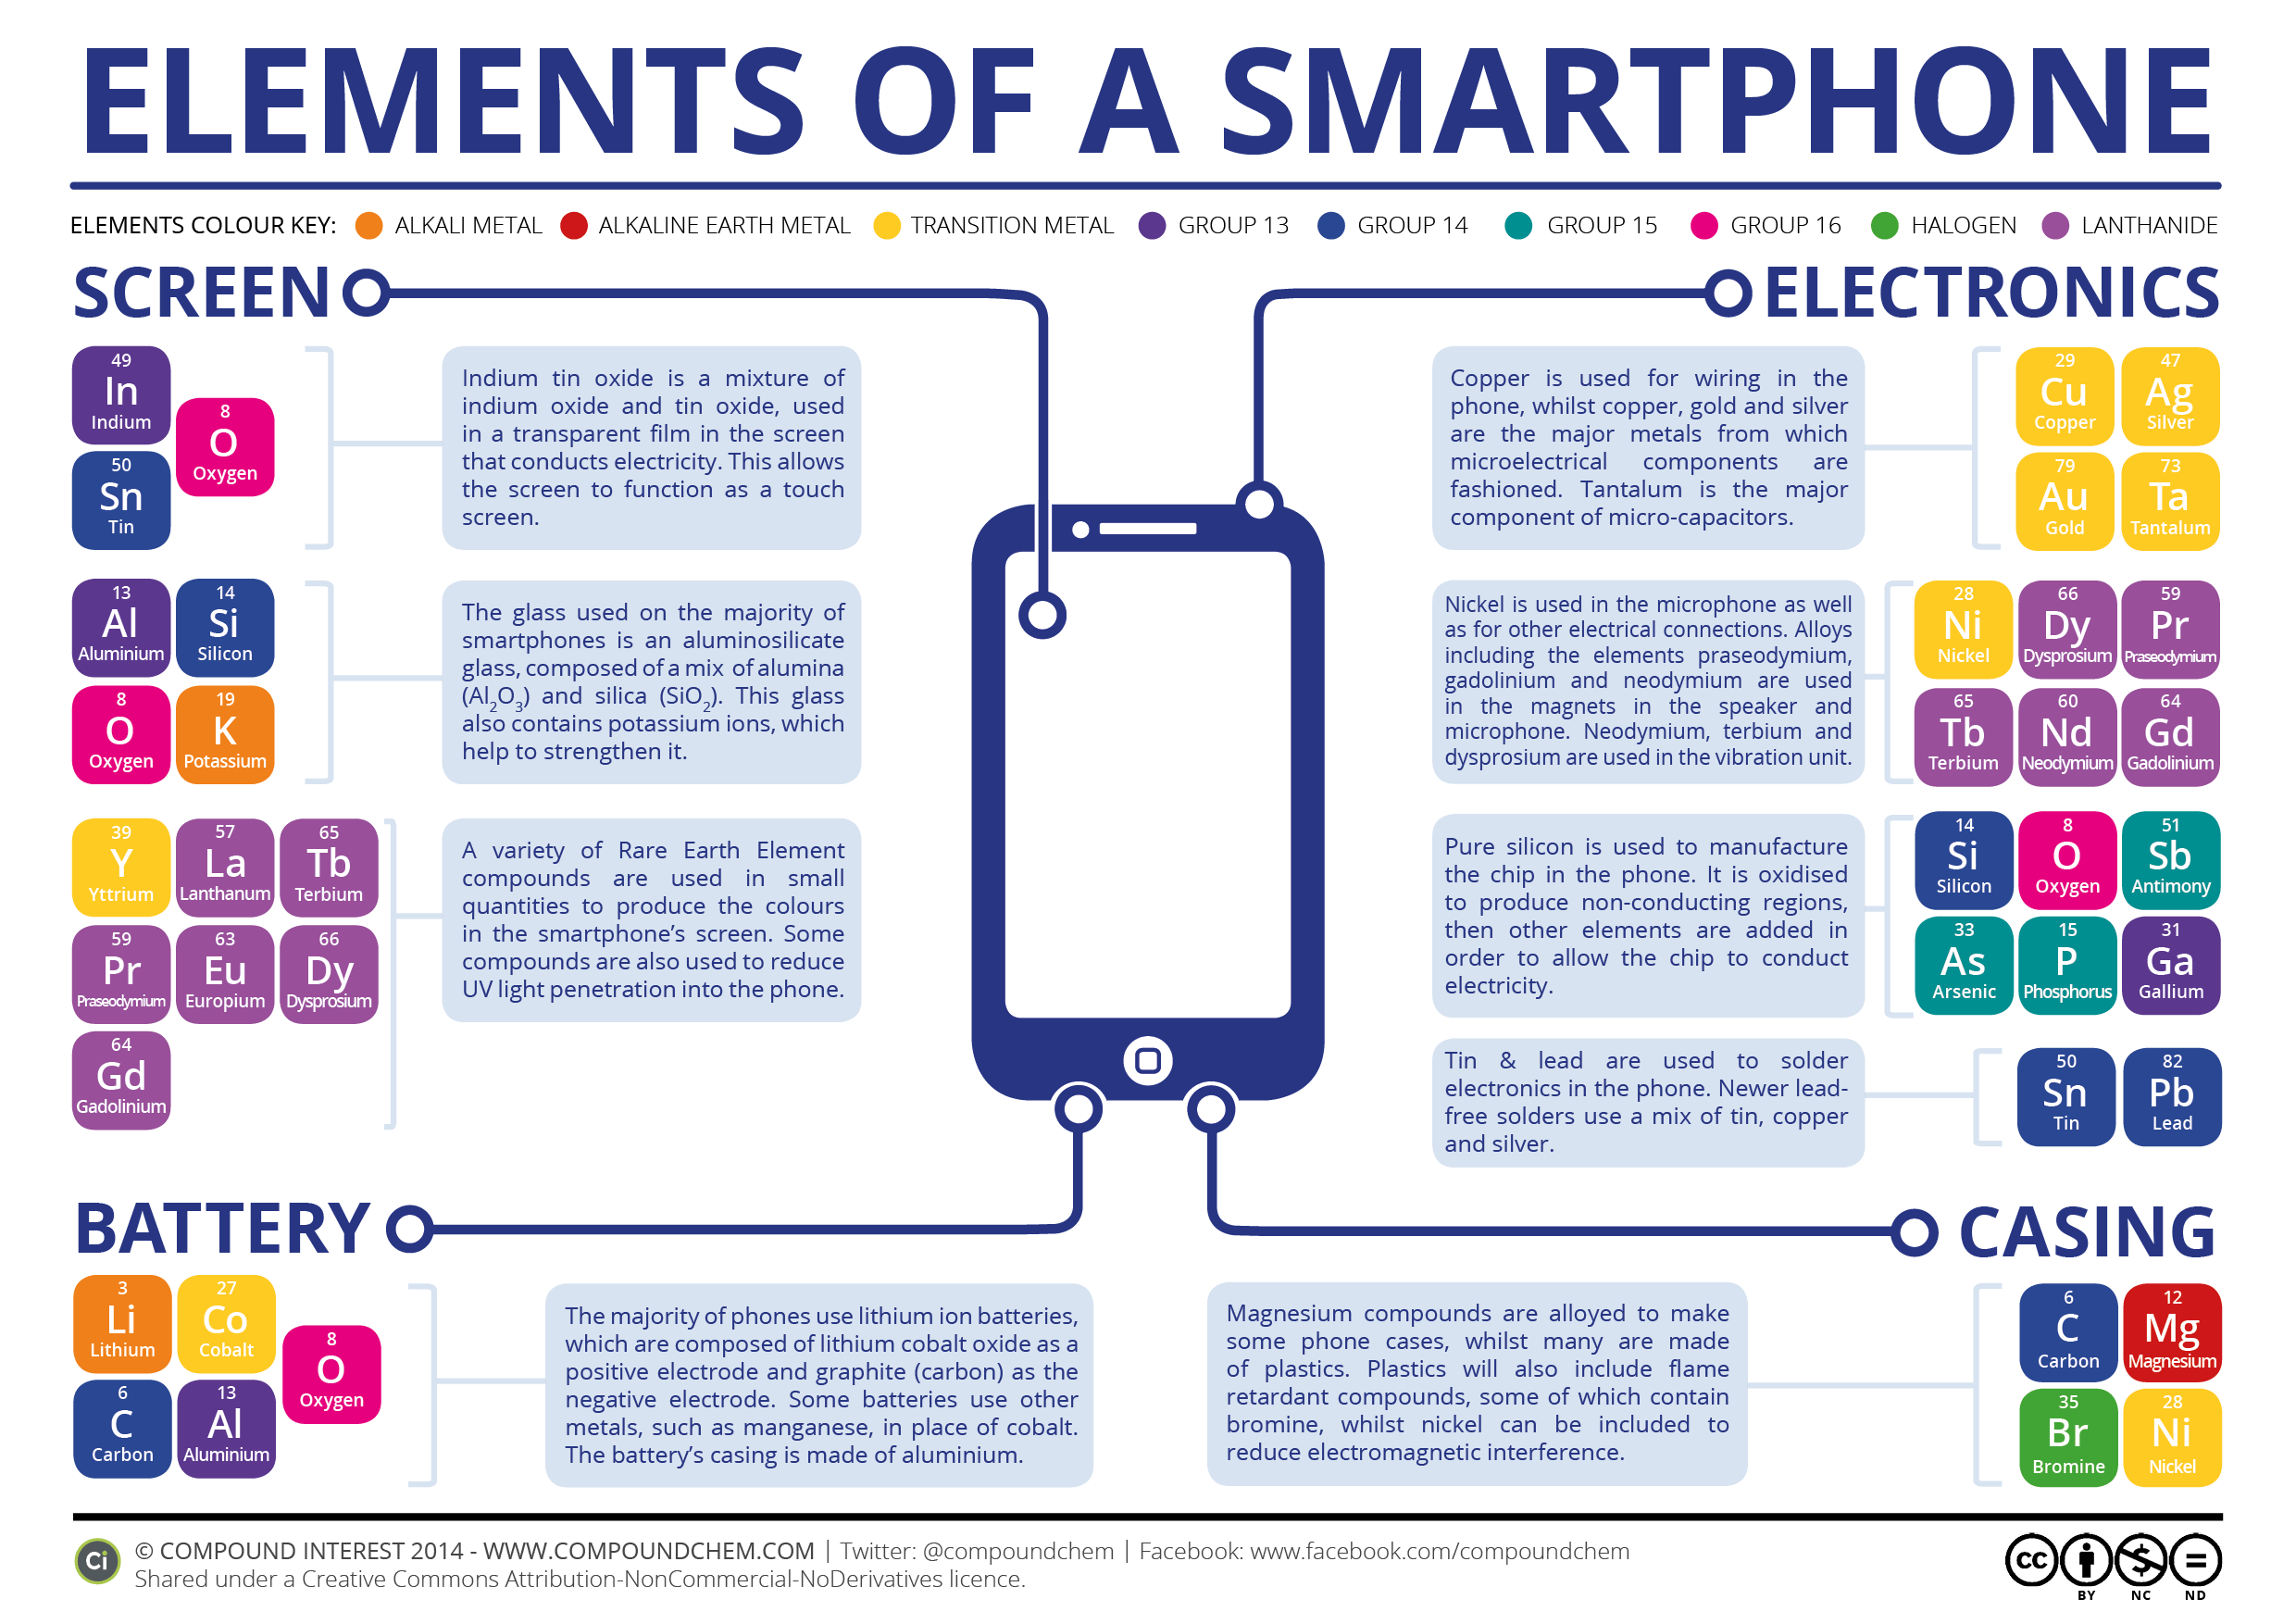
\includegraphics[width=.95 \textwidth]{./images/elements_of_smartphone.png}
    \centering
    \caption{Elements of a smartphone, broken down by its screen, electronics, battery and casing. The official name for Rare Earth Elements (REE) is Lanthanides (denoted by light purple colour) \cite{compoundinterest2014}.}
    \label{ELements_Of_Smartphone}
\end{figure}

A scarce mineral is one that occurs in low abundance or is geologically scarce. Often these are ``hitch-hikers" mined along with more abundant minerals. Gold and palladium are scarce metals that are essential for smartphones and are used in the microelectrical components \cite{compoundinterest2014, geologicalsociety2018}. In contrast, critical metals are not necessarily scarce; instead they have a high economic importance and a high risk associated with their supply. This supply risk is a combination of many factors, including substitutability, end-of-life recycling rates (see Section \ref{SECTION_RECYCLING}), and a high geographical concentration of production in countries with poor governance \cite{eu2014criticalmaterials}. Examples of these critical metals include cobalt (battery), indium (touch screen), tantalum (micro-capacitors) and rare earth elements (colours in screen, magnets in speaker and microphone, vibration unit) \cite{peiro2013material, compoundinterest2014}.

The supply of rare earth metals ($>90\%$) are almost completely controlled by China \cite{schulz2018critical, physorg2012scarcemetals}, with 31\% just in the town of Bayan Obo. As well, China contains the vast majority of the world's reserves of indium which is essential to the production of screens \cite{reller2009mobile, eu2014criticalmaterials}. For the batteries, the majority of mobile devices use lithium batteries. Over 80\% of the world's lithium deposits are found in Chile, Argentina and Bolivia \cite{reller2009mobile}. Tantalum is the major component of micro-capacitors and four fifths of the world's supply is contained in Africa, of which 80\% is in the Democratic Republic of Congo (DRC) \cite{nzongola2002congo, montague2002stolen}. Australia and Brazil also contain high reserves of Tantalum, but the majority of the supply comes from the DRC due to the the lack of safety and environmental standards reducing extraction costs \cite{aspi2013tantalum}. China also contains large reserves of Tantalum, but are choosing to preserve them for the time being \cite{humanityaction2015tantalum}. The DRC also supplies just over half of the world's supply of cobalt \cite{eu2014criticalmaterials}, a component essential for modern batteries.

Substitutes may be found for these materials in the future, although this is unlikely. These minerals are essential for the production of ICT devices and so the potential for geopolitical and economic disruptions to these reservoirs is non-trivial.

%%%%%%%%%%%%%%%%%%%% Environmental Impact %%%%%%%%%%%%%%%%%%%%%%%%%%%%%%
\subsubsection{Environmental Impact}
The five stages in the life of a mine are \cite{hartman2002introductory}
\begin{enumerate}
    \item \textbf{Prospecting}: searching for ores or other valuable minerals. This is typically performed by direct (physical geologic studies, aerial photography, satellite) and indirect (geophysics, geochemistry, geobotany) prospecting methods. Impacts at this stage tend to be minimal, with some land disturbance.
    \item \textbf{Exploration}: determining the extent and value of the mineral deposit. From here a feasibility study is created in order to determine whether to abandon or develop the mine. Again, impacts at this point are minimal with some land disturbance.
    \item \textbf{Development}: opening a mineral deposit for exploitation. Preliminary development work typically consists of acquiring water and mineral rights, buying surface lands, arranging for financing, permit applications and preparing an environmental impact statement (EIS). Construction of access roads, mineral transport systems, mineral processing facilities, waste disposal areas, offices and other support facilities is then done. Depending on whether the minerals are to be mined at the surface or underground, the appropriate excavation method is performed. In surface mining, you must first strip the overburden, which is the waste material (soil, rocks, and living organisms) overlying the desired mineral product. Typical stripping ratios (ratio of waste rock removed to ore recovered) vary between materials and mining sites. For underground mining, these are generally much more complex and expensive; they consist of a carefully planned layout of access openings for mining. Due to the cost, surface mining is the dominant exploitation method worldwide: almost all non-metalic minerals ($>95\%$), most metallic minerals ($>90\%$) and the majority of coal ($>60\%$) are mined by surface methods \cite{ramani2012surface}. This stage has a substantial environmental impact due to the land disturbance (typically deforestation), water pollution and production of wastes.
    
    \item \textbf{Exploitation/Production}: the recovery of the minerals from the earth in quantity and the processing of them to separate the economically valuable minerals from their ores. For surface mining, aqueous methods and mechanical excavation methods (including open pit, strip mining, and mountaintop-removal mining) are typically employed \cite{lima2016legacy}; for underground mining, unsupported, supported and caving are used. In the ore processing phase, the valuable minerals are separated from the ore to yield a higher grade product (i.e. the higher the desired ore grade, the more waste produced). This results in a multitude of wastes, including contaminated mine water, tailings (a fine-grained mineral sand waste) and a variety of chemicals. With a few metals being the exception, the environmental impacts of mining are dominated by this purification and refining stage \cite{nuss2014life}.
    
    \item \textbf{Reclamation}: closure and restoration of the mining site. The best time to begin the reclamation process is before the first excavations are initiated so that the overall cost of mining plus reclamation is minimized (rather than just the cost of mining). One concern that needs to be addressed is the the sealing of openings and the removal of office buildings, processing facilities, transportation equipment, utilities and other surface structures. The other chief concern is the restoration of the land surface, water quality and waste disposal areas. These goals tend to range from the avoidance of exposure to pollutants (remediation) to the full recovery of the original ecosystem (restoration). Unfortunately, restoration is typically unachievable due to the mining site's altered hydrology, habitat fragmentation, contamination, climate change and prohibitive costs \cite{lima2016legacy}.
\end{enumerate}

%Of the 30 billion tonnes of ore and waste materials mined each year, surface mining is responsible for 25 billion tonnes \cite{ramani2012surface}

A major legacy of surfacing mining is the waste left behind. The extraction of 12 billion tonnes of ore is associated with the extraction of 19 billion tonnes of waste \cite{copco2007mining}. In the development stage, a large volume of waste rock needs to be excavated to reach the ore body (the amount of which depends on the stripping ratio). This waste rock is often stored nearby in piles or heaps. Since the composition of these waste rocks varies, the elements leached into the environment also varies. Some elements are highly toxic even in small concentrations (for example, mercury), while others are less toxic but still pose a risk in higher concentrations (copper and zinc) \cite{geointro}.

In the exploitation stage, the tailings waste is typically uneconomical to remediate and so is stored in a slurry form and permanently contained behind a tailings dam to protect the surrounding environment. These tailings damns are some of the largest structures built by geotechnical engineers \cite{lyu2019comprehensive}. For reference, the Baotou tailings dam in Bayan Obo covers 11.5 km$^2$ and contains 150 million tonnes of tailings \cite{pan2016investigating}. In the reported 18,000 mines worldwide, the failure rate in the past one hundred years is approximately 1.2\%, which is two orders of magnitude greater than the 0.01\% failure rate of conventional water retention dams \cite{icold2001tailings}. A comprehensive review of over 300 tailing dam failures worldwide found that the major causes were seepage (21.6\%), foundation failure (17.3\%), overtopping (20.6\%), earthquake (17.0\%) and other (23.5\%). Although many accidents are related to natural events such as heavy rain and earthquakes, each failure also involved engineering and human factors which could have been avoided \cite{lyu2019comprehensive}. When these failures occur they have a significant negative impact  on the ecosystems and human settlements downstream \cite{hudson2003impact}. Another issue that is more commonplace is the long-term leaching of tailings contaminants into the surrounding water and land systems \cite{guo2013leaching}.

Using data back to the 1800s, we see an exponentially increasing trend for mining production, an exponentially increasing trend for waste rock and a gradual declining trend of ore grades. These ore grades are unlikely to ever increase in the future; in the case of gold, its ore grade is expected to decrease by half in the near future \cite{mudd2007sustainability}. An in-depth life cycle analysis of specific metals is conducted in \cite{nuss2014life}. In their periodic table of global warming potentials (GWPs), the GWP per kilogram of each element\footnote{For reference, carbon dioxide has a GWP of 1} is 12,500 for gold, 3,880 for palladium, 260 for tantalum, 196 for silver, 102 for indium, 17.1 for tin and 12.6 for the REE tungsten.

%removal of the surface cover over the deposit, the changes to the original topography, the effects on soil and hydrologic conditions, the issues of mining and processing wastes, and the effect on the future economic potential of the mined areas and communities \cite{ramani2012surface}

%%%%%%%%%%%%%%%%%%%%%% Rare Earth Elements %%%%%%%%%%%%%%%%%%%%%%%%%%%%%
\subsubsection{Rare Earth Elements}
The global demand for rare earth elements---used in ICT devices, modern military equipment and green technologies such as wind turbines, solar panels and hybrid vehicles---is continually increasing, resulting in a rapid growth of REE production and consumption. In addition to the challenges already mentioned, REE often ``hitch-hike" with radioactive elements (for example, thorium, uranium and radium) due to their similar chemical and physical attributes. The result is radioactive tailings and radioactive enrichment around REE mining and processing sites \cite{huang2016protecting} that may lead to growth inhibition, cytogenetic effects and organ‐specific toxicity to abiotic and biotic systems \cite{pagano2015health, zhang2000chronic}.

There are over 1,000 identified REE deposits worldwide; however, only a few of them are being actively mined. In 2011, China produced approximately 95\% of REE materials, with the Bayan Obo mine in Northern China being the largest \cite{huang2016protecting}. Known as the ``death village", the surrounding village of Dalahai have experienced widespread intoxication of the farmland, animals and humans, including respiratory illnesses, cardiovascular disease, leukemia and cancer as a result of the mine \cite{huang2016protecting, eja2020bayanobo, dailymail2011bayanobo}. The potential geopolitical implications of this REE monopoly have been felt and is a source of concern \cite{gulley2018china, zhang2015did}, especially in the aftermath of China's sudden suspension of REE to Japan over a border dispute in 2010 \cite{ting2013rare} and now in 2021 as China explores limiting the export of REE to the USA that are crucial for their military \cite{financialtimes2021REE}.

%%%%%%%%%%%%%%%%%%%%%% Conflict Minerals %%%%%%%%%%%%%%%%%%%%%%%%%%%%%%%
\subsubsection{Conflict Minerals} \label{SECTION_CONFLICT_MINERALS}
Conflict minerals are natural resources that are extracted in a conflict zone and are used to fund the fighting. A prominent example are minerals that originate from the DRC or adjoining states and are processed into tin, tungsten, tantalum and gold (3TG) \cite{fitzpatrick2015conflict}, all of which are used in smartphones \cite{compoundinterest2014}. The Second Congo War (or Africa's First World War) was a devastating 6-year conflict involving at least six nations in the region. Characterized by extreme violence, mass population displacements, widespread rape and a collapse of public health services, the conflict resulted in the deaths of approximately 3.9 million people from 1998 to 2004 \cite{coghlan2006mortality}. %Despite being the largest humanitarian disaster in recent decades, there has been little response from the international community
Although the war has officially ended, it has since given way to a lower-intensity conflict in the eastern provinces of the DRC that continues to take a toll on the people living in the region \cite{coghlan2009update, cfr2021congoconflict}

Although a complex conflict with many narratives and underlying systematic structures outside the scope of this paper\footnote{As due diligence, we thought it imperative to mention the importance of not exclusively focusing on one cause of and one solution to the violence in the DRC. By focusing only on this single narrative, this has diverted attention from essential policy actions, the fight against corruption and the reform of the state administration; inadvertently this has exacerbated the very violence that proponents of this narrative were trying to reform \cite{autesserre2012dangerous}. Due to the scope of this paper, however, we will not be going into this further and we have instead given the reader an assortment of excellent resources that do.}
\cite{autesserre2012dangerous, alorse2015assessing, grant2015new}, one narrative we will focus on is the illegal exploitation of mineral resources that funds the conflict and perpetuates the violence (also referred to as the resource curse). Four fifths of the world's supply of tantalum comes from Africa, of which 80\% is in the DRC \cite{nzongola2002congo, montague2002stolen}. Despite 110 years of mineral extraction (untapped deposits are estimated to be worth \$24 trillion USD \cite{cfr2021congoconflict}), the wealth has not been used to better the citizens of the DRC; rather it has gone to the country's rulers and their political and business partners in the international community \cite{nzongola2002congo}. According to the United Nations' 2020 Human Development Index, the DRC ranks 175 out of 189, with 64\% of their population living in poverty \cite{unitednations2020hdr}.

For the trace mineral tantalum, ICT devices consumed approximately 15\% of global shipments and this total was estimated to increase to 27\% by 2018 \cite{fitzpatrick2015conflict}. For a more in-depth discussion of the tantalum supply chain, please see \cite{mancheri2018resilience}.

%%%%%%%%%%%%%%%%%%%%%% Conflicting Solutions %%%%%%%%%%%%%%%%%%%%%%%%%%%
\subsubsection{Conflicting Solutions}
Solutions to conflict minerals have been difficult due to the many complex interactions at play. Policy solutions tend to aim for the goal of certifying minerals as conflict-free or initiatives for conflict-free sourcing. These include the Organisation of Economic Co-Operation and Development (OECD) Due Diligence Guidance \cite{oced2016duediligence}, the United Nations (UN) Guiding Principles on Business and Human Rights \cite{un2011guidingprinciples}, the European Union (EU) Conflict Minerals Regulation \cite{ec2020duediligence} and the industry led Conflict-Free Smelter Program (CFSP) \cite{cfsi2016cfsp}. As well, extractive taxes in Chile \cite{anrc2016chilecasestudy} and Norway \cite{lund2014state} have allowed the countries to mostly avoid the resource curse. Lessons from these countries may yield insights for how resource-rich countries manage their mining revenue.

At a legislative level, the United States passed a provision of the Dodd-Frank Act in 2010 to prevent the purchase of conflict minerals by compelling USA companies to audit their supply chains. Although well-intentioned, this unfortunately had unintended consequences. Due to the complex supply chains in the DRC \cite{moran2015global, reller2009mobile}, this has made it difficult for companies to determine if the supply is conflict free which has resulted in many multinational companies no longer buying from the DRC. This caused many miners to lose their jobs and their families to fall deeper into poverty, driving some to join the very armed militia groups the Dodd-Frank Act was attempting to target \cite{cfr2021congoconflict}. For DRC territories with an average number of gold mines, the passing of the Dodd-Frank Act increased the incidence of battles by 44\%, looting by 51\% and violence against civilians by 28\%. This provision of the Dodd-Frank Act pertaining to conflict minerals (Section 1502) was repealed in 2017 \cite{stoop2018more}. 

From 2004 to 2014, there has been a 250\% increase in unaccounted production from small scale and artisanal mining \cite{mancheri2018resilience}. Officially, the DRC did not report any export of tantalum in 2013 or 2014. However, the import data from other countires shows 517 tons of tantalum was imported from the DRC. A discrepancy in Rwanda shows that 2,466 tons of tantalum were exported in 2013 but the country only produced 600 tons. This gap in official production numbers likely arises from rebel groups in the DRC smuggling tantalum across the border into Rwanda and Uganda where it is then exported \cite{mancheri2018resilience}.

%%%%%%%%%%%%%%%%%%%%%%%%%%%%%%% Cobalt %%%%%%%%%%%%%%%%%%%%%%%%%%%%%%%%%
\subsubsection{Cobalt}
Although not part of the 3TG conflict minerals in the eastern DRC, the southern region of Katanga supplies 60\% of the world's cobalt (no other country produces more than 6\% \cite{shedd2017cobalt}) which is essential for lithium-ion rechargable batteries in your phone, computer and electric vehicles. Due to the relative level of peace in Katanga compared to the eastern provinces of the DRC and the mines not being controlled by armed rebel groups, the mines here are not seen as ``conflict minerals". There is however widespread instability, violence and minimal rule of law surrounding the mines \cite{scheele2016cobalt}.

The formal industrial cobalt mines in the DRC are controlled by Congolose state-owned and foreign companies \cite{scheele2016cobalt}, with China having a major influence \cite{gulley2019china}. These companies have been associated with labour rights violations, community conflicts and land grabs \cite{scheele2016cobalt}. Studies have also found that people living within 3 km of industrial mines and smelters have high levels of exposure to cobalt and other trace elements \cite{banza2009high}. In the last three decades, there has been a growth of local residents participating in the artisanal and small-scale mining (ASM) sector. Although the share of cobalt from ASM is difficult to determine due to its informal and often illegal nature, an estimated 15-20\% of cobalt in the DRC is extracted this way \cite{al2017cobalt}. Widespread child labour is employed here \cite{andre2014child} and despite the potentially fatal health effects of prolonged exposure to cobalt \cite{nkulu2018sustainability}, adult and child miners often work without basic protective equipment, including gloves, work clothes or masks.  Artisanal miners manually dig their own mines, often extending far underground without any supports and poor ventilation, resulting in the frequent collapse of unsupported tunnels \cite{al2017cobalt, amnesty2016drc}. Once extracted, the ores are sold to traders who then sell it to Chinese, Indian, or Lebanese companies who then export them to cobalt refining countries including China, Belium, Finland and Canada \cite{al2017cobalt}.


%%%%%%%%%%%%%%%%%%%%%%%%%%%%%%%%%%%%%%%%%%%%%%%%%%%%%%%%%%%%%%%%%%%%%%%%
%%%%%%%%%%%%%%%%%%%%%% End of Life Emissions  %%%%%%%%%%%%%%%%%%%%%%%%%%
%\cleardoublepage
\subsection{E-Waste} \label{SECTION_END_OF_LIFE_EMISSIONS}
 \begin{fquote}[Case Study from Heftingsdalen, Norway][Vital Waste Graphics 2 \cite{bournay2006vital}]
 For consumers, waste disappears the moment their bin is emptied. They see us as a sort of cemetery for the consumer society. They completely disregard the concept of waste and what it becomes. Nor do they have much idea of the many ways waste may be processed. Nothing disappears. It all becomes something else, which inevitably impacts on our environment and way of life...Five years ago waste processing plants represented a fairly effective, sustainable solution, now they are a crisis response.
 \end{fquote}

E-waste\footnote{E-waste is also known as Waste Electrical and Electronic Equipment (WEEE), a term mostly used in Europe. The e-waste statistics used in this section include ICT devices as well as other electronic and electrical equipment (e.g., basic kitchen appliances, toys, lamps, and tools for music).} are the electrical and electronic equipment (EEE) and its components that have been discarded as waste without any intention of reuse (Figure \ref{e-waste}). In 2019, the world generated an astounding 53.6 Mt\footnote{1 metric megaton (Mt) is equivalent to 1,000,000,000 kilogram (kg).} of e-waste, which averages to 7.3 kg per person. And this number is projected to increase with a doubling time of 16 years: by 2030, the world is projected to create 74.7 Mt of e-waste. This growth is not distributed equally, however. Although Asia generated the most amount of e-waste, per capita Europe is the highest with each citizen producing an average of 16.2 kg of e-waste. This is followed by similar levels in Oceania (16.1 kg per capita) and the Americas\footnote{Within certain regions, there is even more variation. For example, Northern America (Canada and the USA) produce 20.9 kg per capita and have a recycling rate of 15\%, whereas Central America (including Mexico, Guatemala and Costa Rica) only produce 8.3 kg per capita with a recycling rate of 3\%.} (13.3 kg per capita). Asia and Africa have by far the lowest, with 5.6 and 2.5 kg per capita, respectively. For a comprehensive breakdown of global and regional e-waste statistics, legislation and health impacts, please see \cite{forti2020global}.

\begin{figure}[h]
    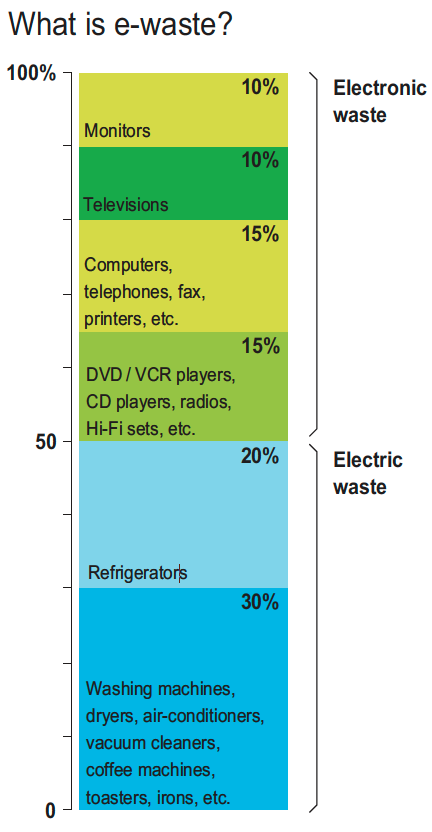
\includegraphics[width=.35 \textwidth]{./images/e-waste.png}
    \centering
    \caption{Components of e-waste. Additional categories not included in this infographic include: lighting equipment (fluorescent tubes); toys, sports and recreational equipment; electric and electronic tools (drills, sewing machines, lawn mowers, etc); surveillance and control equipment; medical instruments; and automatic ticket machines \cite{bournay2006vital}.}
    \label{e-waste}
\end{figure}

The major factors enabling this increased consumption of ICT devices globally are higher levels of disposable income, growing urbanization and mobility, and further industrialization \cite{forti2020global}. In addition to this higher consumption rates of ICT devices, shorter product life cycles (Section \ref{SECTION_PLANNED_OBSOLESCENCE}) and few repair options (Section \ref{SECTION_RIGHT_TO_REPAIR}) means that more of these devices are becoming e-waste sooner (Figure \ref{Global_e_waste_stats}). Since we discussed these factors contributing to e-waste in previous sections, please refer back to them if you require a refresher.

Much of this waste is classified as hazardous due to its component metals, the use of halogenated flame retardants to reduce flammability and the compounds generated or used during the recycling process \cite{williams2011environmental, forti2020global}. In addition to the valuable metals of copper, gold and silver in an ICT device, you also have an assortment of hazardous metals including lead (soldering), antimony and arsenic (chip) \cite{compoundinterest2014, williams2011environmental}, mercury (background lights of older displays and televisions) \cite{balde2018waste}, cadmium (rechargeable batteries)  \cite{williams2011environmental, forti2020global} and lithium (lithium batteries) \cite{compoundinterest2014, kumar2017waste}.

\begin{figure}[h]
    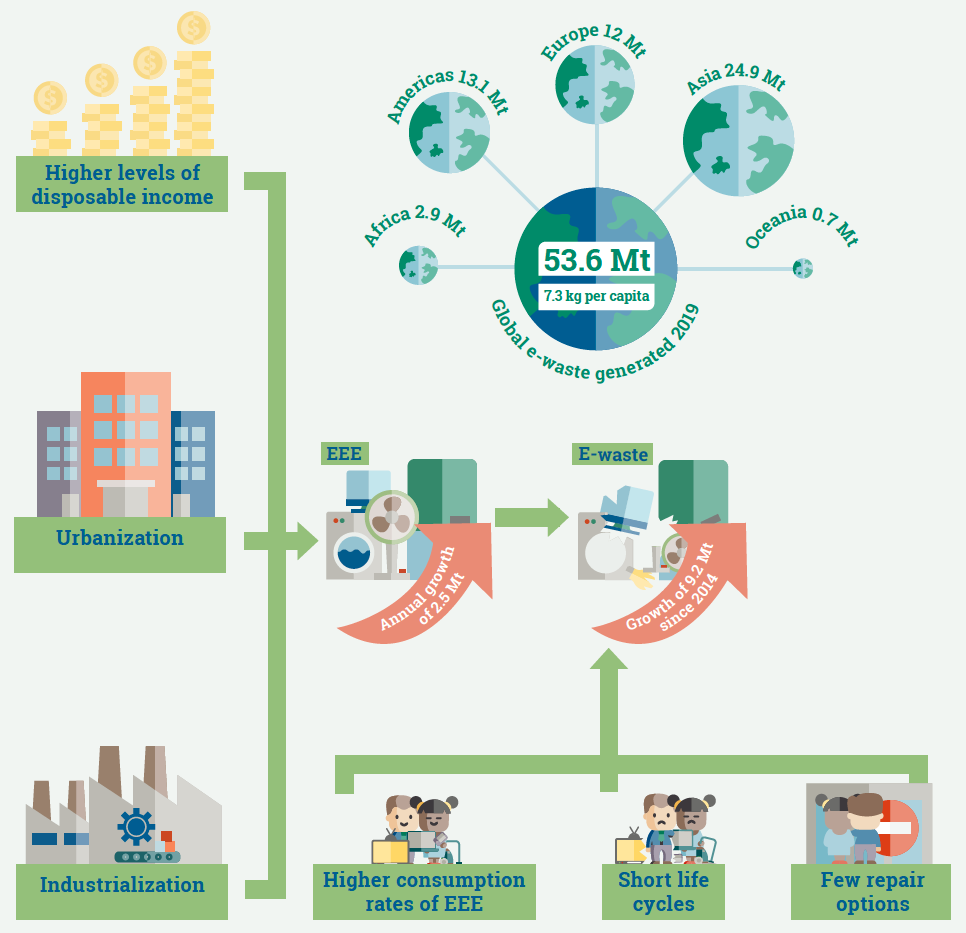
\includegraphics[width=.75 \textwidth]{./images/e-waste_global.png}
    \centering
    \caption{Global production of e-waste broken down by regions, as well as the major contributing factors for the growth of the electrical and electronic equipment (EEE) consumption and the growth of its subsequent e-waste \cite{forti2020global}.}
    \label{Global_e_waste_stats}
\end{figure} 
 
 %%%%%%%%%%%%%%%%%%%%%%%%%%%%% Recycling %%%%%%%%%%%%%%%%%%%%%%%%%%%%%%%%
\subsubsection{Recycling} \label{SECTION_RECYCLING}
 Not all discarded ICT devices will end up in recycling centres. The fate of 82.6\% (44.3 Mt) of generated e-waste in 2019 was unknown: we know neither its whereabouts nor do we know its environmental impacts. This is troubling because many abandoned devices contain hazardous elements that may leach into the environment \cite{forti2020global}. Mercury can enter the food chain and accumulate in living organisms, resulting in damage to the central nervous system, thyroid, kidneys, lungs, immune system and irreversible brain damage \cite{balde2018waste}. Unfortunately, this improper management of e-waste results in a sizeable amount of raw materials not being recovered \cite{forti2020global}. Rather than using recycled materials to substitute for primary raw materials, we must extract and refine virgin material deposits (Section \ref{SECTION_ACQUISITION_RAW_MATERIALS}) for our new products. Similar to the generation of e-waste, the recycling rates are not evenly distributed across the globe. In 2019, Europe had the highest rate at 42.5\%, followed by Asia (11.7\%), the Americas (9.4\%), Oceania (8.8\%), and Africa (0.9\%) \cite{forti2020global}.

%%%%%%%%%%%%%%%%%%%%%%%%% Recycling Rates %%%%%%%%%%%%%%%%%%%%%%%%%%%%%%%
% \cleardoublepage
\subsubsubsection{How Recyclable are my Recyclables?} \label{SECTION_HOW_RECYCLABLE_ARE_MY_RECYCLABLES}
Let's say you are one of the lucky ICT devices that does make it to a (formal or informal) recycling center. Even if an ICT device is recycled, there is a significant variation between the recycling rates of each metal (Figure \ref{Recycling_Rates_Smartphone}). In the case of rare earth elements, you have a less than 1\% recycling rate; often it is not economically possible to retrieve these trace metals because the amounts used are so small \cite{physorg2012scarcemetals, habib2015tracking}. And so we risk irretrievable dissipation of these elements into the biosphere, rendering them impossible for reuse \cite{reller2009mobile}. Although the critical metal cobalt has a $>50\%$ recycling rate, the other critical metals of indium, tantalum and all of the rare earth elements have a $<1\%$ recycling rate \cite{compoundinterest2014}. Within 1 tonne\footnote{1 tonne is equivalent to 1,000 kilograms or 1,000,000 grams.} of mobiles phones, there are 280 grams of gold \cite{forti2020global} (for comparison, the gold ore grade is lower at approximately 5 grams of gold per 1 tonne of ore) \cite{mudd2007sustainability}. Since newer phones are being manufactured with less gold, they require less raw materials. But they are also less profitable to recycle and so the gold contained within them is often not recovered \cite{geyer2010economics}. For the plastic components, the outlook is not much better. Of the seven billion tonnes of plastic waste that humanity has generated so far, an estimated 10\% were recycled, 14\% were incinerated and the remaining 76\% are either in landfills, dumps or the natural environment \cite{geyer2020production}. These poor recycling rates unfortunately puts additional stress on supply chains.

\begin{figure}[h]
    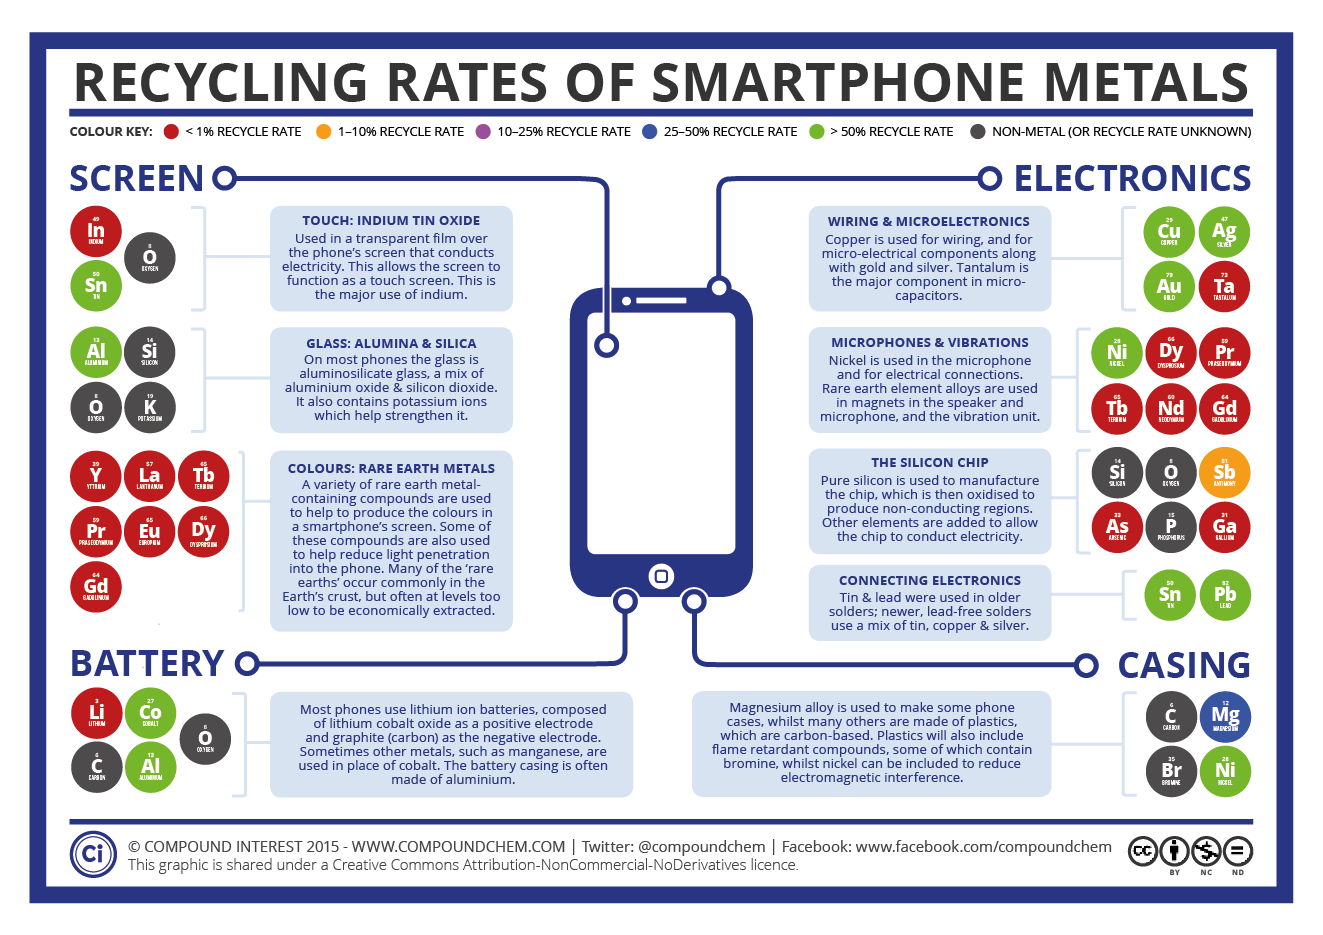
\includegraphics[width=1 \textwidth]{./images/recycling_rates_of_smartphone.png}
    \centering
    \caption{Recycling rates of a smartphone, broken down by its screen, electronics, battery and casing \cite{compoundinterest2014}.}
    \label{Recycling_Rates_Smartphone}
\end{figure}

Let's say you are also one of the lucky percentages that did get recycled. There is still another obstacle you may face on your path to being truly recyclable: the vast majority of recycling today is actually downcycling. When a material is recycled, they are often mixed with other materials to produce a hybrid of lower quality therefore making them suitable only for applications of lower value. Rather than creating a circular cradle-to-grave dynamic, their trip to the landfill has only been slowed. This is problematic for metals since the rare earth elements and valuable minerals are blended in the recycling process, thus making their discrete value lost forever \cite{braungart2007cradle}. Downcycling is also problematic for plastics which make up approximately 50\% of a smartphone, most of which is contained in the case and circuit boards \cite{bournay2006vital}.

When recycling, it is often difficult to separate the hazardous wastes from the valuable material. An example of this are the halogenated flame retardants found in the outer casings of computers, circuit boards, wires and cables in order to reduce flammability \cite{williams2011environmental, forti2020global}. When this e-waste is recycled into waste plastic it can then be used in lower grade applications, including plastic kitchen equipment. Despite European legislation prohibiting polybrominated diphenyl eithers (PBDEs) and hexabromocyclododecane (HBCD) in food contact articles, studies have shown that halogenated flame retardants are present in black thermos cups and black plastic kitchen utensils \cite{samsonek2013occurrence}.

%%%%%%%%%%%%%%%%%%%%%% Waste Colonialism %%%%%%%%%%%%%%%%%%%%%%%%%%%%%%%
\subsubsubsection{Not in My Backyard}
% This also got me thinking about waste colonialism —it’s a concept that describes the transboundary movement of waste largely overseas transferring waste and its burdens from high GDP nations to low GDP nations -- not only does the Global North place the blame on marginalized individuals but also the burdens

Unwanted ICT products may still be refurbished and reused and so they are often shipped from higher income countries to lower income countries, whom may or many not have a fully developed e-waste management infrastructure. Although some ICT devices extend their life cycle this way, a sizeable amount of e-waste generated is illegally shipped under this guise \cite{forti2020global}. %Despite having e-waste recycling infrastructure, high-income countries export a sizeable portion to developing countries. 

The 1970s and 1980s saw a rise of environmental regulations to properly handle hazardous wastes in developed countries, resulting in a higher cost for e-waste disposal. In developing countries (and some developed countries) there are fewer safety regulations, lower cost of labour and a strong demand for raw materials in transitioning economies. Since developed countries could no longer dump their unwanted hazardous materials in a local landfill, it became more economical for them to load these wastes onto ships and trains, transport them beyond their regulated jurisdictions and dump them in another backyard for a fee. The result was a massive trans-boundary flow of e-waste from developed countries to developing countries such as China, India and Pakistan  \cite{sthiannopkao2013handling, zhang2012waste}.

In response to this digital dumping situation, the 1992 Basel Convention on The Transboundary Movement of Hazardous Wastes and their Disposal banned this toxic trade of hazardous wastes, including e-waste \cite{baselconvention2011}. Although a comprehensive agreement that charged countries to be responsible for the safe disposal of the hazardous wastes they produced, it did not extend to functioning second-hand goods \cite{sthiannopkao2013handling}. Despite China\footnote{Upon resuming sovereignty of Hong Kong, the Basel Convention also applied to the Hong Kong Special Administrative Region.} ratifying the Basel Convention in 1991 \cite{baselconvention2011ratify}, the illegal smuggling of e-waste continued to pour in. The New Territories region of Hong Kong was a major e-waste trafficking port of landing; from here it was then smuggled across to mainland China \cite{ban2018carecyclingexport}. To stop the illegal export of waste from other countries, China began enforcing strict border controls in 2013 (Operation Green Fence) and even stricter measures in 2017 (National Sword). Although it successfully reduced the illegal waste accepted at the Chinese border, it had unfortunate cascading effects. Rather than developed countries reducing or processing all of their waste, the problem has been shifted to yet another backyard \cite{financialtimes2018nationalsword}. Much of the rejected waste has ended up in other Southeast Asian countries and Pakistan (Figure \ref{e-waste_china_import}), many of whom lack the infrastructure to manage their own waste, much less the additional waste from the developed world \cite{ban2018carecyclingexport, brooks2018chinese}.

\begin{figure}[h]
    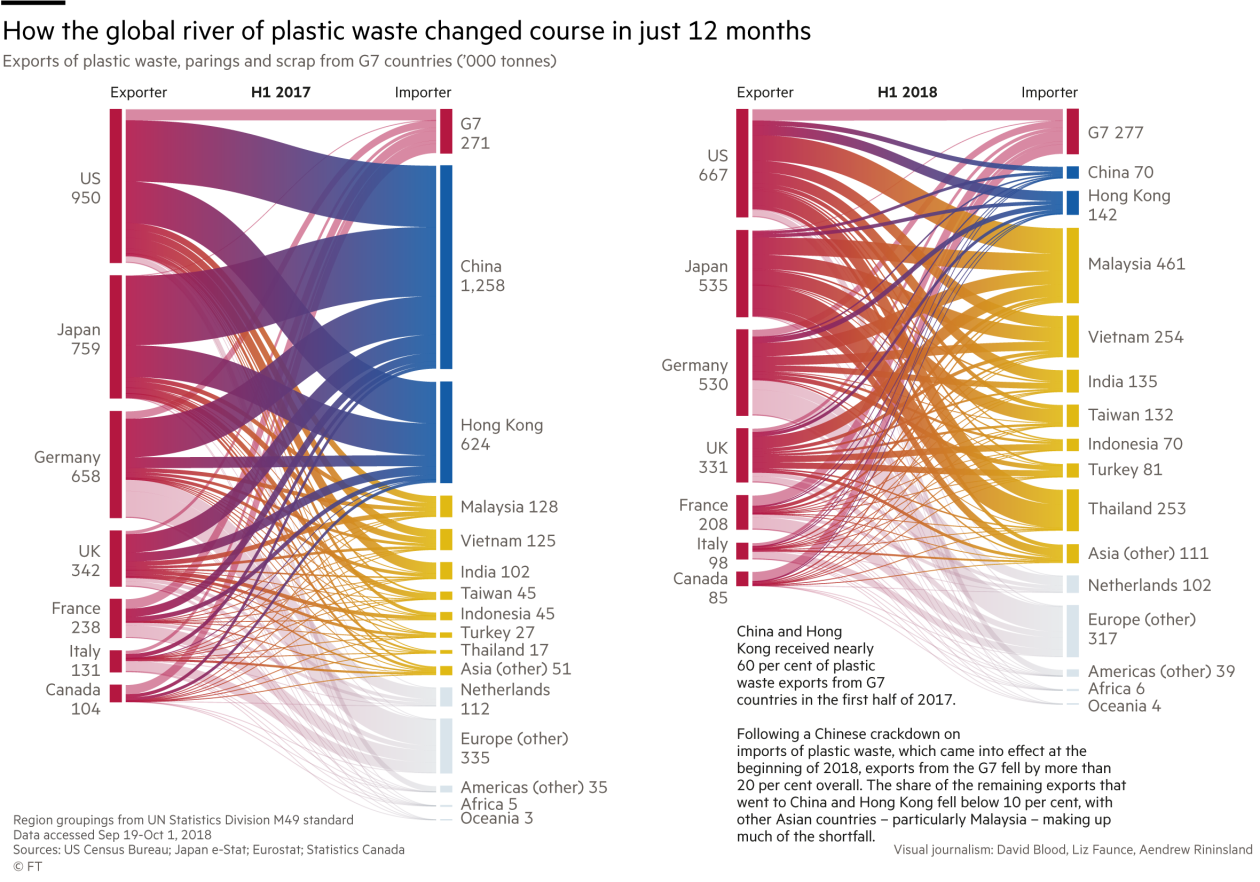
\includegraphics[width=.95 \textwidth]{./images/e-waste_china_import.png}
    \centering
    \caption{\textit{The import and export of plastic waste from G7 countries before and after China's National Sword \cite{financialtimes2018nationalsword}.}}
    \label{e-waste_china_import}
\end{figure}

A 2016 study using Global Positioning System (GPS) trackers found that 34\% of the USA's e-waste were exported, with the majority going to Hong Kong (Figure \ref{US_export_e-waste}) \cite{ban2016usrecyclingexport}. A similar 2018 study in Canada found a 16\% export rate of recyclers \cite{ban2018carecyclingexport}. Although better, it is still concerning since Canada has a legal obligation under the Basel Convention, while the USA does not \cite{baselconvention2011ratify}. 

\begin{figure}[h]
    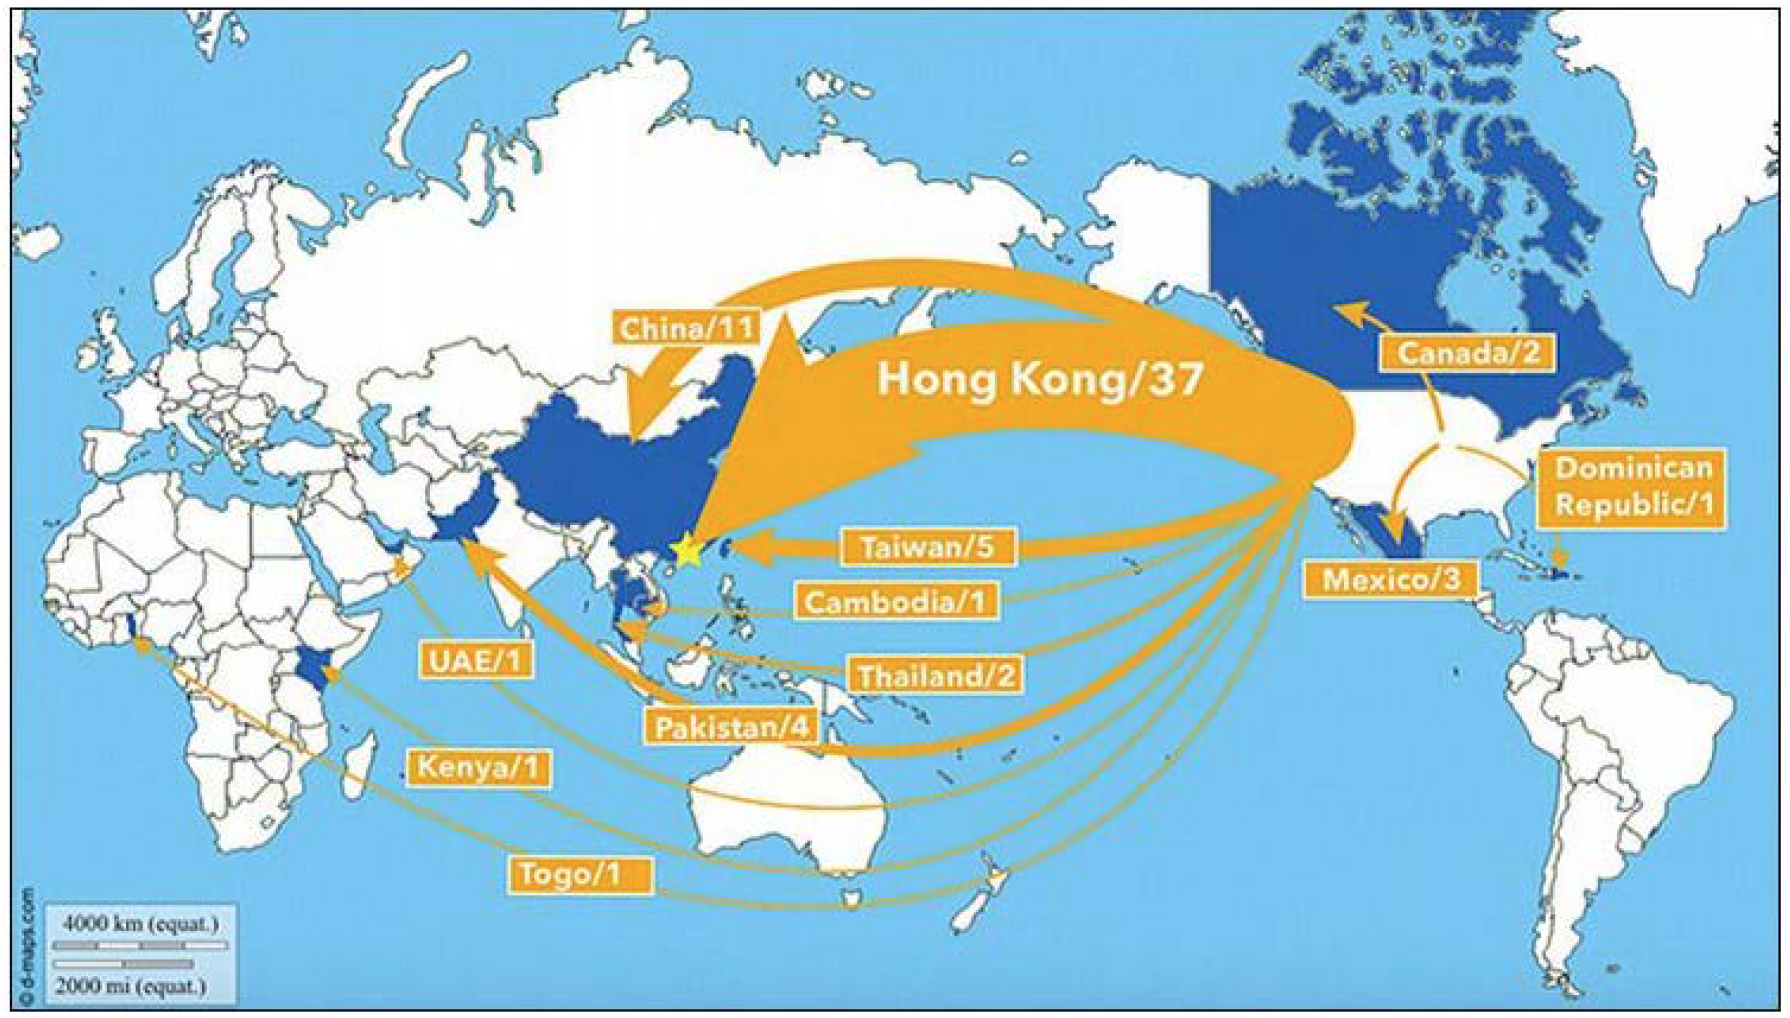
\includegraphics[width=.8 \textwidth]{./images/US_export_e-waste.png}
    \centering
    \caption{A map showing the destinations of the electronic products tagged with trackers in the e-Trash Transparency Project \cite{ban2016usrecyclingexport}.}
    \label{US_export_e-waste}
\end{figure}

When we throw our waste ``away", away becomes ``here" for someone else. A framework for viewing this transboundary movement is \textit{waste colonialism}: developed nations use their dominance (or hegemonic power) to exploit the land of developing nations for waste disposal. Blame is then attributed to developing nations' poorer waste disposal systems and international emissions accounting reinforces this by allowing developed nations to export their e-waste emissions\footnote{The international community takes a production-based approach to measuring a country's emissions: a country is responsible for the emissions associated with the extraction of raw materials, production of goods and disposal of waste within their borders. This system forms the basis of the United Nations Framework Convention on Climate Change (UNFCCC) international carbon accounting systems and efforts to mitigate carbon emissions, including the Kyoto Protocol and the Paris Agreement \cite{unfccc2009kyoto, unfccc2015paris}. This accounting decision means a country's emission reduction commitments do not include emissions attributed to their imports---essentially, countries are allowed to export their emissions.} \cite{tukker2020consumption, wang2007owns}. Consequences of waste pollution disproportionately impacts those who are least responsible for the pollution and who are least able to mitigate the effects \cite{liboiron2018plastic, pratt2010decreasing}.

%%%%%%%%%%%%%%%%%%%%%%%%%%% Formal Recycling %%%%%%%%%%%%%%%%%%%%%%%%%%%
\subsubsubsection{The Formal Recycling Sector}
The formal recycling sector is typically established by national e-waste legislation. E-waste is collected by designated organizations, producers or the government (often through retailers, collection points or pick-up services) and it is taken to dismantling facilities \cite{forti2020global}. In the first step, hazardous materials are separated from electronic devices, which are further dismantled into their plastic, glass, wires and electrical components. During the end-processing stage, the wires and electronics are sent to a smelter to recover the valuable metals which are then purified in refineries \cite{kumar2017waste}. Meanwhile the plastic components are melted down for re-use in lesser applications, in a process known as downcycling \cite{braungart2007cradle}. Wastes from this process are either incinerated or held in controlled landfills. This formal recycling process should be performed in accordance to the country's e-waste legislation, which typically mandates the proper handling of hazardous wastes and protection of the health of workers and the environment \cite{forti2020global}. Despite these health and safety regulations, damage to the environment, the health of the workers and surrounding populations are still an issue (Section \ref{SECTION_RECYCLE_ENVR_IMPACTS}).

Although higher-income countries tend to have a waste recycling infrastructure, around 8\% of e-waste still ends up in waste bins. Consequently this e-waste is treated like regular mixed household wastes. These are typically incinerated (Europe) or landfilled (Canada and most of the USA) without material recycling or the safe handling of hazardous elements \cite{forti2020global}. 

%%%%%%%%%%%%%%%%%%%%%%% Informal Recycling %%%%%%%%%%%%%%%%%%%%%%%%%%%%%
\subsubsubsection{The Informal Recycling Sector}
Since many middle- and low-income countries have an e-waste management infrastructure that is not fully developed or entirely absent, e-waste is often managed by the informal sector. The informal sector is typically characterized by small-scale, labour-intensive, low-technology recycling that is unregulated and unregistered. It is often carried out by poor and marginalised social groups who must resort to scavenging and waste picking in order to generate income---sometimes for everyday survival. Although informal recycling is typically regarded in a very negative light, %---it is backward, unhygienic and incompatible with modern waste management systems---
it is a rather efficient recycling system that can improve recycling rates and it provides a livelihood for a major section of the urban poor \cite{wilson2006role, medina2000scavenger}.

The collection phase of used products and e-waste can be identified into at least four main categories: 1) door-to-door buying, bartering or collecting; 2) street waste picking from litter or communal bins before collection; 3) municipal waste collection crews recovering materials from the vehicles on the way to disposal sites; and 4) waste picking from dump sites \cite{wilson2006role}. Once collected, the products are sold to be repaired, refurbished or informally recycled. Within the recycling phase, dismantlers manually break the e-waste into usable components and materials, using simple tools or their bare hands. For components that are no longer functioning but still contain valuable materials, recyclers will burn, leach and melt the e-waste to recover the secondary raw materials \cite{forti2020global}. Since they are encased by a plastic cover, cables are openly burnt to remove the plastic and recover the valuable copper. This is usually done a short distance from where the dismantling is performed due to the toxic smoke generated \cite{akormedi2013working}. Similarly, computer casings are ``cooked" to remove the combustible plastics and to isolate the metals. To release the chips, circuit boards are de-soldered by grilling them over an open fire to melt the lead and plastic. Once released, the chips are placed in open-pit acid baths to leach the gold and other metals. These wastes may then be directly disposed into nearby fields, rivers and irrigation ditches \cite{chan2013review, sthiannopkao2013handling}. This lack of safety regulations and equipment exacerbates the challenges of recycling, causing severe damage to the environment and the health of the workers and surrounding populations (Section \ref{SECTION_RECYCLE_ENVR_IMPACTS}).

\begin{figure}[h]
    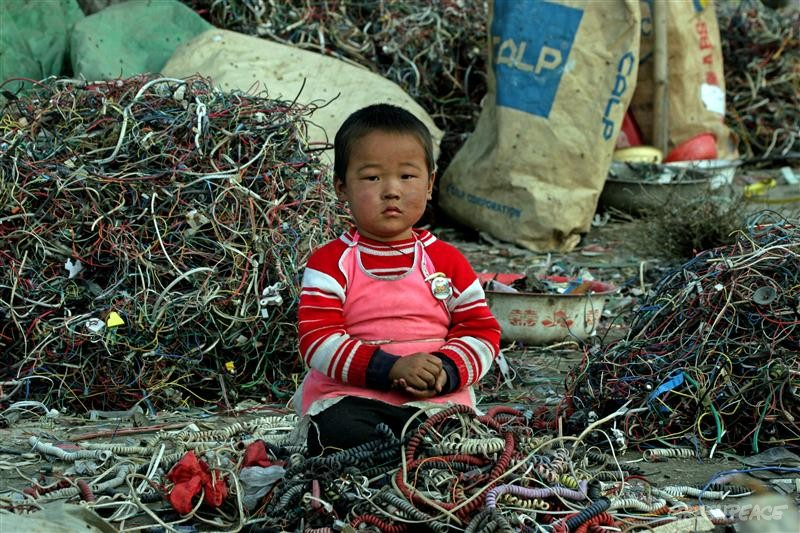
\includegraphics[width=.8 \textwidth]{./images/e-waste_guiyu.png}
    \centering
    \caption{A small child sitting among cables and e-waste in the informal recycling sector in Guiyu, China \cite{greenpeace2005guiyuewaste}.}
    \label{guiyu_e-waste}
\end{figure}

One of the most notorious case studies of informal recycling is the town of Guiyu in southeast China which processed over 20 million tonnes of e-waste in 2004 alone. There were more than 5,500 shops informally employing over 30,000 people, many of whom were children, for an average wage equivalent of US\$1.50 per day \cite{chi2011informal, chan2013review}. Most workers laboured without goggles, proper ventilation or other basic personal protective equipment \cite{sthiannopkao2013handling}. In 2015, China closed down Guiyu's informal sector and forced all e-waste processors in the area to either quit or relocate to the new industrial park. Although a major step towards enforcing China's e-waste importation ban and improving the local environmental and human health, e-waste smugglers have simply found new backyards to dump their e-waste to be informally processed. Shortly after, concerns began to arise over the New Territories in Hong Kong becoming the next Guiyu \cite{ban2018carecyclingexport}.

%%%%%%%%%%%%%%%%%%%  Human & Environmental Impacts %%%%%%%%%%%%%%%%%%%%%
\subsubsubsection{Environmental \& Human Health}\label{SECTION_RECYCLE_ENVR_IMPACTS}

%%%%%%%% Informal %%%%%%
Many hazardous compounds enter the surrounding ecosystem by direct dumping into water systems, fumes and dust entering the atmosphere and soil, and the leaching of substances from landfills, incinerators and recycling \cite{williams2011environmental}. From here they may enter the water and food systems through the livestock, fish and crops (Figure \ref{e-waste_ecosystem_contamination}). Although workers---especially those without personal protective equipment---have direct exposure, the surrounding community will still be exposed through dietary intake, soil and dust ingestion, inhalation and dernal contact  \cite{williams2011environmental, chan2013review}. Unregulated e-waste recycling has been associated with a myriad of adverse human health effects, including prenatal exposure causing adverse birth outcomes \cite{xu2012birth}, limited or delayed growth and development of children \cite{liu2018thyroid}, decreased learning outcomes \cite{soetrisno2020chronic}, damaged DNA \cite{alabi2012comparative}, changes to cardiovascular regulation \cite{cong2018elevated}, decline in lung function and an increased risk for asthma and chronic obstructive pulmonary disease (COPD) \cite{amoabeng2020effect}, weakened immune systems \cite{zhang2017alteration}, hearing loss \cite{xu2020hearing} and cancer \cite{davis2019strong}.

\begin{figure}[h]
    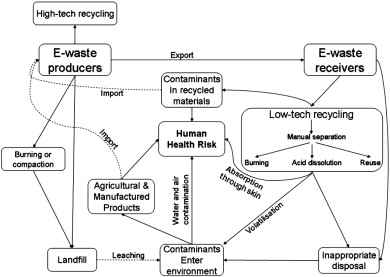
\includegraphics[width=.8 \textwidth]{./images/e-waste_ecosystem_contamination.jpg}
    \centering
    \caption{Exposure routes and behaviour of e-waste toxicants from producers to receivers and ultimately to humans \cite{robinson2009waste}.}
    \label{e-waste_ecosystem_contamination}
\end{figure}

%%%%%%%%% Formal %%%%%%%%%
Although the formal sector has safety regulations and protective equipment for workers, the concentration of hazardous compounds and exposure is still adverse for workers and the surrounding community. In a study of Canadian e-waste workers, certain air concentrations, dust concentrations and worker exposures in formal indoor facilities exceeded those of informal indoor e-waste facilities in low and middle income countries. Possible explanations included the facilities being contained in a large but enclosed indoor facility (with a poor ventilation rate) and a lack of operating emission abatement equipment \cite{nguyen2019exposure, nguyen2020can}. Workers performing recycling tasks in Sweden's formal e-waste facilities had significantly higher concentrations of toxic metals including chromium, cobalt, indium, lead and mercury \cite{julander2014formal}. Community exposure is also a problem for the towns surrounding formal recycling facilities. The Horne smelter in Canada is North America's largest recycler of electronic components and is one of the world's largest producers of copper and other precious metals. To the residents' surprise, it was announced at a 2019 town hall meeting that the lead and arsenic levels in their children were 3.7 times higher than children living in a nearby town. In response, the company owning the smelter has added more domes to manipulate the process within a closed environment instead of outdoors; there was no comment on the impact of this on indoor air concentrations, dust concentrations or worker exposure. Although better than open burning, since 1993 the Horne Smelter has released 936,000 kg of arsenic and 2,710,000 kg of lead according to the federal database of pollutants \cite{cbc2019hornesmelter}.

%Children attending school within a 2.5 kilometers radius of a smelter had higher levels of lead within their blood. As well, lead in school-playground dust and lead on children's hands were correlated to the lead in the air \cite{roels1980exposure}.

%%%%%%%%%%%%%%%%%%%%%%%% Legislative Solutions %%%%%%%%%%%%%%%%%%%%%%%%%
\subsubsection{Searching for Solutions}
\begin{fquote}[Dr. Max Liboiron][How Plastic Is a Function of Colonialism \cite{liboiron2018plastic}]
Disposability is not the result of the bad behavior of some individuals choosing to buy some things and not others. Consumer choice as a concept makes no sense in many places. In Nain [the most northern Inuit community in Nunatsiavut, Canda], there is one store. There is one kind of ketchup you can buy. There is one type of lettuce. Both are in plastic packaging because the producers assume that there is a place for that packaging to go. It goes into the dump, where it is usually burned so bears aren't attracted to town, and then the scraps blow into the water. There is no way to behave differently. Bag bans don't eliminate the problem. Degradable plastics made of corn would move the problem onto someone else's land. Shipping Nain's plastics to a recycling plant in Vietnam or even elsewhere in Canada produces pollution and plastic leakage on other lands still. Disposable plastics are simply not possible without colonizer access to land.
\end{fquote}

%%%%%%%%%%%%%%%%%%%%%%%%%%%% Rethink %%%%%%%%%%%%%%%%%%%%%%%%%%%%%%%%%%%
\subsubsection*{\textit{Rethink}}
Rather than band-aid solutions that temporarily mask our e-waste problems, we need to take a systematic approach by rethinking our current processes, policies and actions to make meaningful change \cite{zerowastecanada2017hierarchy}. At this highest level of the Zero Waste Hierarchy (Figure \ref{zero_waste_hierarchy}), we need to make fundamental changes to our product designs. For example, we could design our ICT products for disassembly and easy separation, use single rather than composite materials and coatings and expand product manufacturer's responsibility to include the full life cycle of their products (also known as extended producer responsibility). By providing incentives for manufacturers to design products that are easier to recycle, reuse and have reduced material usage, the environmental impact of a product across its life cycle can be reduced \cite{walls2006extended}.

\begin{figure}[h]
    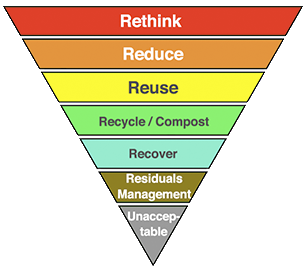
\includegraphics[width=.5\textwidth]{./images/zero_waste_hierarchy_crop.png}
    \centering
    \caption{Canada's Zero Waste Hierarchy \cite{zerowastecanada2017hierarchy}.}
    \label{zero_waste_hierarchy}
\end{figure}

On an individual consumer level, we can also rethink how we choose the ICT devices that we buy. Rather than purchasing ICT devices based on the more typical metrics of initial costs or the latest trends, you could also base your decision on other metrics (circumstances permitting). Other potential factors to consider are the device's embodied emissions, its lifespan, durability, repairability, reusability, or multifunctionality. However, not everyone will have the privilege to access or base their decisions on more long-term considerations \cite{boddy2016telling} nor does individual action at the end of the pipeline address the underlying systemic issues. As well, consumer choice as a concept does not make sense in many places and for many individuals \cite{liboiron2018plastic}. As well, the rise of the conservation movement has a long history baked in privilege, power and racism; this is beyond the scope of the paper but if you are interested we strongly recommend reading further \cite{taylor2016rise, purdy2015environmentalracism}.

An interesting piece of research by \cite{ryen2014community} tried to examine what more green ICT design would look like. By adapting biological ecology models to analyze the dynamic structure and function of the ICT device community, future strategies to encourage more green design and consumption of ICT devices should focus on minimizing the total number of products. One way to achieve this is by maximizing each device's multifunctionality with convergent device design.

%%%%%%%%%%%%%%%%%%%%%%%%%% Reduce & Reuse %%%%%%%%%%%%%%%%%%%%%%%%%%%%%%
\subsubsection*{\textit{Reduce \& Reuse}}
We have previously discussed the proliferation of ICT devices, planned obsolescence (Section \ref{SECTION_PLANNED_OBSOLESCCENCE}) and the lack of repair options (Section \ref{SECTION_RIGHT_TO_REPAIR}), so we will not repeat what we have already discussed.

%%%%%%%%%%%%%%%%%%%%%%%%%%%%%% Recycle %%%%%%%%%%%%%%%%%%%%%%%%%%%%%%%%%
\subsubsection*{\textit{Recycle}}
Worldwide only 78 countries had a national e-waste policy, legislation or regulation in 2019. Although this is an improvement from previous years, many regions are struggling with slow regulatory advancements, lack of investment, lack of political motivation and poor enforcement \cite{forti2020global}. Most of these countries have an informal recycling system that is efficient in terms of material recovery, but which is highly damaging to the environment and human health. Rather than scrapping them entirely, developing countries have the opportunity to build upon the existing informal recycling systems or to incorporate them into their formal systems \cite{wilson2006role}.

Recycling infrastructures will vary globally, but there are some universal guiding principles: adequate financing, effective collection and distribution systems, safe facilities for dismantling, safe facilities for separation and purification, regulatory oversight and extended producer responsibility to ensure an effective connection between recyclers and producers \cite{braungart2007cradle, bournay2006vital, forti2020global}.


%%%%%%%%%%%%%%%%%%%%%%%% Concluding Remarks %%%%%%%%%%%%%%%%%%%%%%%%%%%%%
\subsubsection{Can We Recycle Our ICT Troubles Away?}
Of the 53.6 Mt of e-waste produced in 2019, let us for a moment assume the best case scenario of 100\% recycling. What would that look like? We would only be able to recover 25 Mt of raw materials and so there would still be a sizeable amount of irrecoverable waste. Based on the current demand of raw materials for new EEE, we would still require an additional 14 Mt of virgin raw material to be extracted and refined \cite{forti2020global}. Another important aspect is the transport and energy costs associated with recycling. To recycle a tonne of waste, it is estimated that half the cost is transport-related \cite{bournay2006vital}. Although the energy cost to recycle an ICT device may be less than the energy cost to extract and process the identical amount of virgin raw materials, the energy cost is still high---to recycle a tonne of mobile phones takes approximately 7,500 megajoules \cite{navazo2014material}---especially compared to the energy associated with reusing or repairing your device and not buying a new one.

Clearly recycling is an important part to the ICT sustainability puzzle, but it is much further down the Zero Waste Hierarchy since it does not address the core problem \cite{zerowastecanada2017hierarchy}. We must also address the systematic forces driving the rapid proliferation of ICT devices, the lack of repair options and planned obsolescence.

%%%%%%%%%%%%%%%%%%%%%%%%%%%%%%%%%%%%%%%%%%%%%%%%%%%%%%%%%%%%%%%%%%%%%%%%
%%%%%%%%%%%%%%%%%%%%%%%% Energy Consumption  %%%%%%%%%%%%%%%%%%%%%%%%%%%
%\cleardoublepage
\subsection{Energy Consumption of ICT} \label{SECTION_ENERGY_CONSUMPTION}
In the pursuit of Moore's, the industry has not been optimizing for energy efficiency; rather we have been optimizing for performance and profits. However, with the new age of mobile and cloud computing there has become a push for longer battery life \cite{waldrop2016chips} and so energy efficiency is becoming a peripheral focus. For data centers, the bulk of their emissions come from their usage phase \cite{andrae2015global, malmodin2014life, irishtimes2016datacentre}. By 2030 the expected case scenario for ICT electricity consumption is expected to hit over 8,000 TWh/year (Figure \ref{Global_Energy_ICT_components}), which represents 21\% of the global electricity consumption (Figure \ref{Global_Energy_ICT_share}). The largest components of this growth is projected to come from data centers and fixed access networks (FAN), which consist of fixed access wired and fixed access Wireless Fidelity (Wi-Fi). Interestingly, the energy consumed by consumer devices (desktops, monitors, laptops, phones, tablets, televisions, gaming consoles and other television peripherals) has been fairly stable and is projected to decline. This decline is mostly attributed to the substantial shift of electricity usage from consumer devices onto the networks and data centers \cite{andrae2015global}. Although this shift has addressed the battery life of our devices and prolonged Moore's, it has unfortunately increased our overall energy consumption.

\begin{figure}[h]
    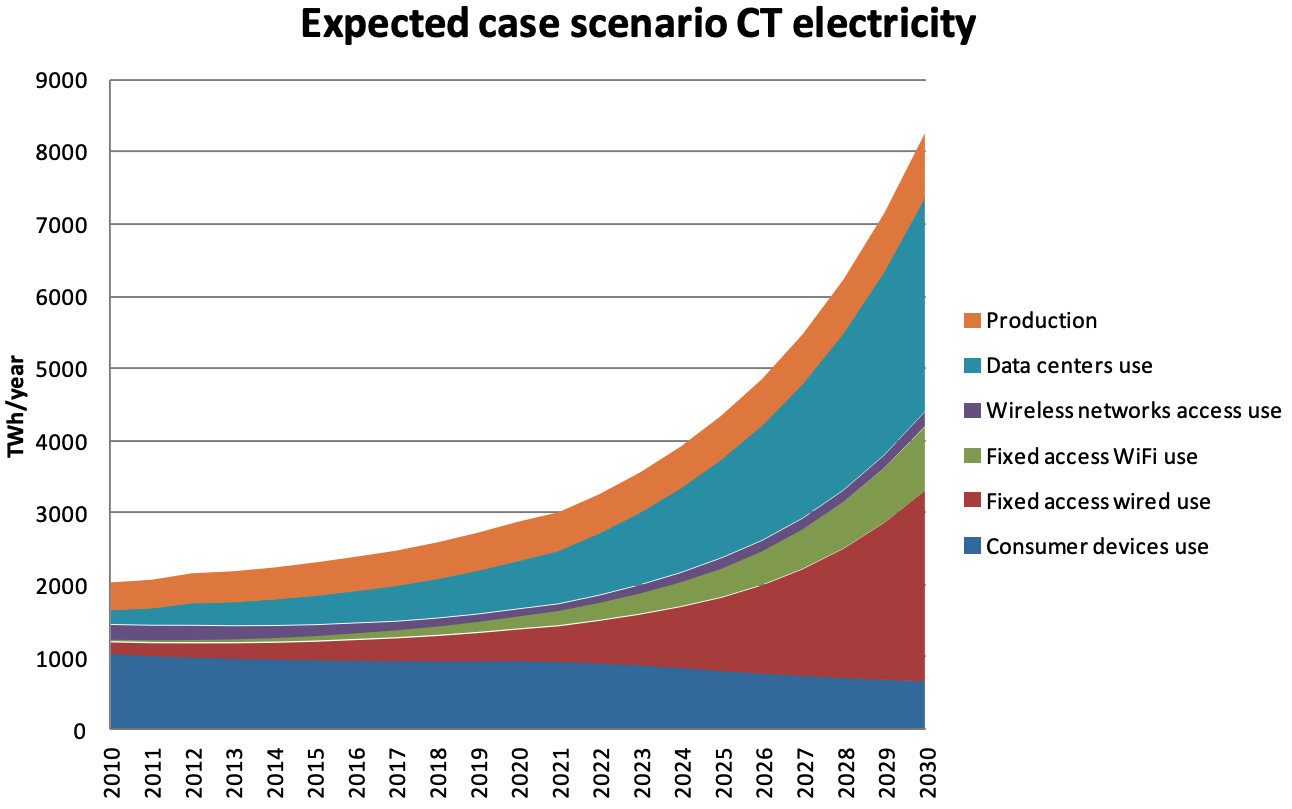
\includegraphics[width=.75 \textwidth]{./images/Global_Energy_ICT_components.png}
    \centering
    \caption{Trends per communication technology (CT) category for expected-case global electricity usage from 2010–2030. The fixed access network (FAN) usage is further broken down into the fixed access wired (red) and fixed access Wi-Fi (green) data traffic. The wireless access networks (WAN, purple) is based on the annual growth of voice traffic and mobile data traffic \cite{andrae2015global}.}
    \label{Global_Energy_ICT_components}
\end{figure}

\begin{figure}[h]
    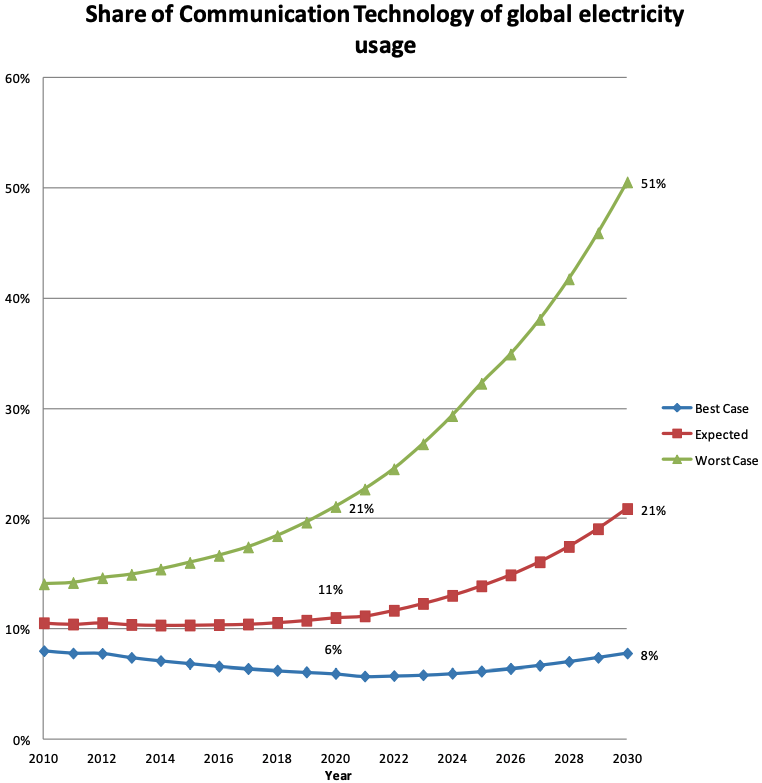
\includegraphics[width=.65 \textwidth]{./images/Global_Energy_ICT_share.png}
    \centering
    \caption{Share of communication technology of global electricity usage 2010–2030 \cite{andrae2015global}.}
    \label{Global_Energy_ICT_share}
\end{figure}

Although many ICT devices are now more energy efficient (for example, television panels have now transitioned to Light Emitting Display (LED) based displays \cite{park2013efficiency}), some newer models use substantially more energy. In November 2020, both Sony and Microsoft released their next-generation home consoles---the Playstation 5 (PS5), the Xbox Series X and the Xbox Series S---which were their most successful launches ever for both companies \cite{cnet2020gamingconsoles}. They give an unprecedented gaming experience of speed, power and graphics, but they are also the most energy-intensive gaming consoles ever made (Figure \ref{usage_gaming_consoles}). For an in-depth life cycle analysis of gaming consoles, please see \cite{aslan2020climate}.

\begin{figure}[h]
    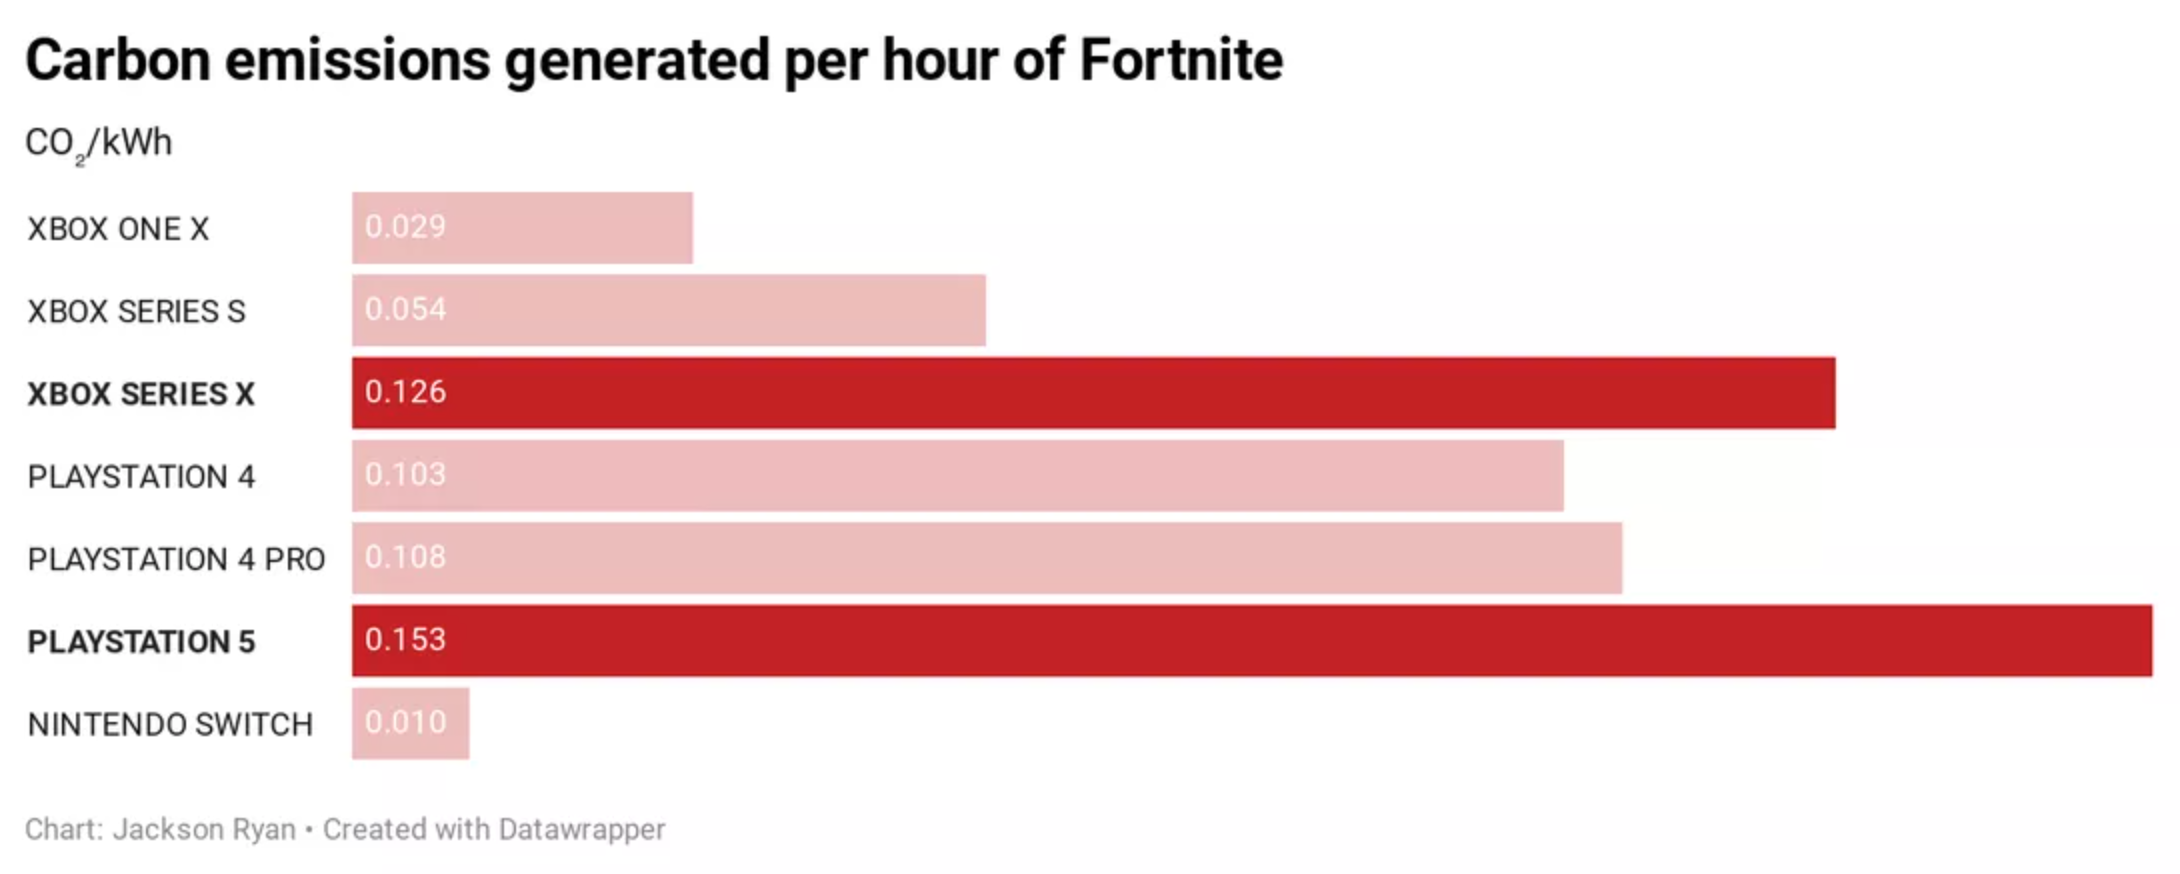
\includegraphics[width=.9 \textwidth]{./images/usage_gaming_consoles.png}
    \centering
    \caption{Comparison of the energy consumption for the newest generation (Playstation 5, Xbox Series X and Xbox Series S) versus the older generations of gaming consoles for a popular game. Note that the new Xbox Series S is the more affordable and less powerful alternative to the Xbox Series X \cite{cnet2020gamingconsoles}.}
    \label{usage_gaming_consoles}
\end{figure}

%%%%%%%%%%%%%%%%%%%%%%%%% Orwellian Energy %%%%%%%%%%%%%%%%%%%%%%%%%%%%%
\subsubsection{Some Energy are More Equal Than Others}
While it is important to measure how much energy a device consumes, it is also crucial to examine how your energy is generated. Depending on whether your energy resources are coming from fossil fuels (coal, oil and natural gas), uranium, renewables (wind, water and solar), waste (for example, waste-to-energy incineration facilities) and/or biomass fuels, the environmental impacts will vary \cite{dincer2000renewable}. Even within a certain category of energy, there is substantial variation \cite{boyle2004renewable}.

A good illustration of this is a study conducted on the operational energy usage of Sweden's ICT network for a single year \cite{malmodin2014life}. In Figure \ref{usage_sweden_global_mix}, we see the carbon footprint of the extended Swedish ICT network is substantially less if computed using Sweden's energy mix (B) versus the same network being powered by the less clean global average electricity mix (C).

\begin{figure}[h]
    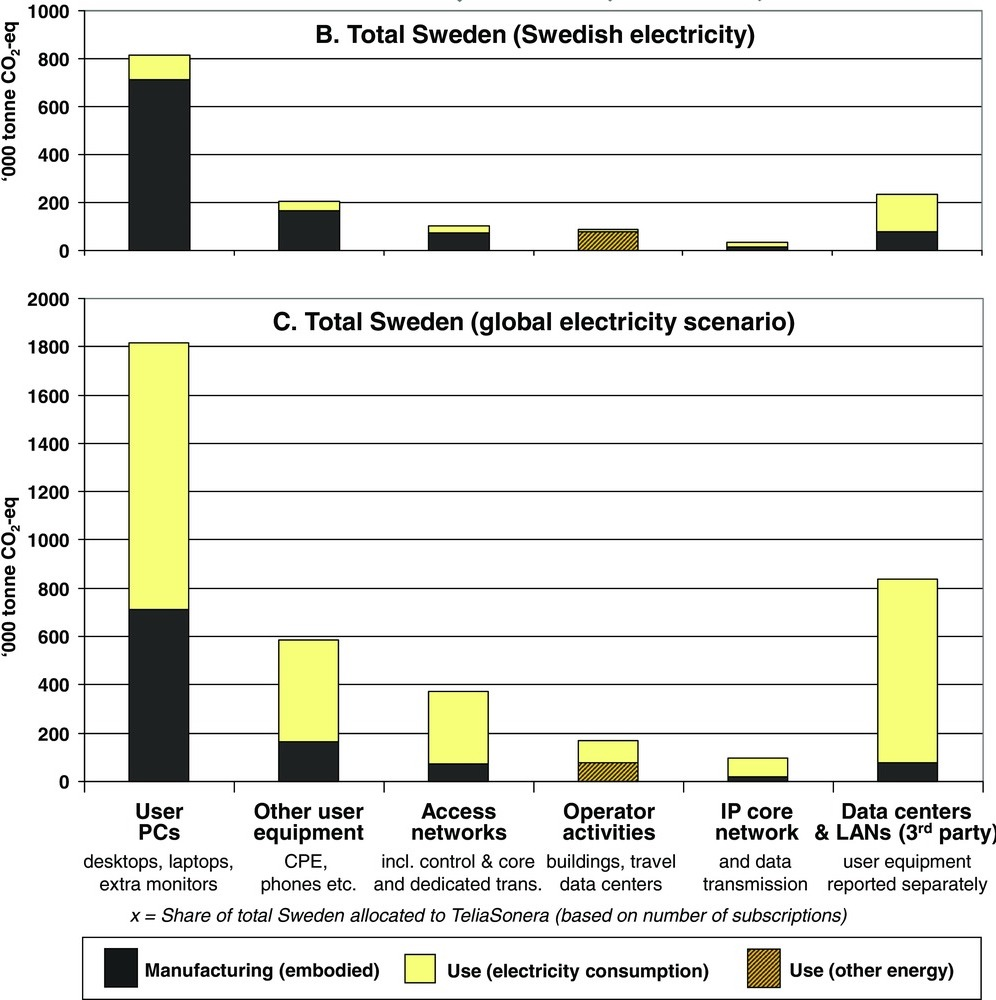
\includegraphics[width=.76 \textwidth]{./images/usage_sweden_global_mix.jpeg}
    \centering
    \caption{Carbon footprint of \textbf{(B)} the Swedish ICT extended network using the Swedish energy mix; and \textbf{(C)} the Swedish ICT extended network using a global energy mix. The carbon footprint is measured in units of carbon dioxide equivalent (CO$_2$-eq). Other acronyms used include Internet Protocol (IP), local area network (LAN) and customer premises equipment (CPE) \cite{malmodin2014life}.}
    \label{usage_sweden_global_mix}
\end{figure}

Although beyond the scope of this paper, if you are interested in the feasibility of providing all worldwide energy from wind, water and solar (WWS) renewables, please see the two part series of \cite{jacobson2011providing, delucchi2011providing}. Interestingly, barriers to covert all power worldwide to WWS renewables are primarily social and political, not technological or even economic.


%%%%%%%%%%%%%%%%%%%%%%%%%%%%%%%%%%%%%%%%%%%%%%%%%%%%%%%%%%%%%%%%%%%%%%%%
%%%%%%%%%%%%%%%%%%%%%%%%%%%% Conclusion %%%%%%%%%%%%%%%%%%%%%%%%%%%%%%%%
%%%%%%%%%%%%%%%%%%%%%%%%%%%%%%%%%%%%%%%%%%%%%%%%%%%%%%%%%%%%%%%%%%%%%%%%
\cleardoublepage
\section{Conclusion} \label{SECTION_DISCUSSION}
 \begin{fquote}[Donella H. Meadows][Limits to Growth: The 30-Year Update \cite{meadows2004limitsupdate}] 
 Running the same system harder or faster will not change the pattern as long as the structure is not revised... Only changing the structure of the system—the chains of causes and effects—will do that.
 \end{fquote}

Now that we have explored each of these biophysical resource limits, the natural question to ask is which limit will bring Moore's exponential growth to a halt? Although intuitive to ask and useful to know, there is a gaping limit to our limits analysis that we have yet to address. Due to the opaque nature of the ICT industry, we lack the data and transparency to quantify which limits we are approaching. It takes me seconds to pull up more specifications than I could ever comprehend for our favourite \$3,000 USD Intel Xeon W-3175X Processor \cite{intel2021processor}, but I cannot tell you how much fossil fuels were required or how much fresh water was used and subsequently polluted in the manufacturing of it. %I can easily tell you Intel Corporation's net income for every year or quarter on the stock market, but after extensive searching I cannot tell you what Intel's carbon footprint was for its fleet of processors or for the company as a whole. 
Stepping back even further, I cannot tell you how much energy, water and fossil fuels the ICT industry consumed, nor what share of the critical metals or REE the industry depleted and recycled. 

Transparency within tech companies has been slowly improving, however. Companies will often have press releases on a very specific aspect of the system (sometimes only when they are pressured to do so \cite{amazon2019openleter}) and many are now releasing environmental reporting on a company or product level. Although standardizing schemes have been developed, they are voluntary and company participation greatly varies. Unlike financial reporting requirements, we do not have government regulations stipulating sustainability transparency and uniformity across the industry \cite{mytton2019sustainabiliytransparency}. And so without a complete picture of the entire system it is nearly impossible to quantitatively pinpoint the limit points %, the leverage points to best intervene in the system, 
and which resource limit will be triggered first. Transparency and data availability is not a silver bullet solution, but it is a pre-condition to effective action.

So what can be done to address the systematic issues plaguing the ICT system? Although pushing for transparency and quantifying these limit points is crucial, we also recommend that future research conducts a leverage points analysis \cite{meadows2008thinking} to identify the points in our global ICT system where we could enact deep, systematic structural change. This analysis consists of identifying points in a system where a small change can lead to a large shift in behaviour. There are 12 leverage points according to Meadows, but for brevity we will cluster them into four groups (in order of increasing effectiveness and difficulty to implement) \cite{penzenstadler2018software}: 
\begin{enumerate}
    \item \textbf{Changing the Metabolic Structure}: fine-tuning how a system works
    \item \textbf{Changing the Feedback Loops}: repercussions of delays in the system and the influence that balancing and reinforcing feedback loops have in maintaining or eroding stability
    \item \textbf{Transformational Change and Self-Adaption}: structure of information flows, rules governing the system and the system's ability to self-organize; and
    \item \textbf{Changing the Intent of the System and Stakeholders}: changing the goals and paradigms of a system
\end{enumerate}

This leverage points analysis, however, is far beyond the scope of this paper, but we will briefly go over the main limit points we have explored and possible questions that it raised. Although most data is undisclosed, we know that manufacturing a single microchip takes an enormous toll on our fresh water reservoirs, fossil fuel emissions and chemical wastes. Thus far we have optimized our manufacturing for computing power and miniaturization, rather than minimizing our environmental impact. This has resulted in incredibly powerful, microscopic chips that are also incredibly damaging to the environment. For the overall ICT device and cloud infrastructure, we have also been optimizing for performance and profits---not energy efficiency. New ICT devices are typically more energy efficient but many newer models are significantly more powerful and so consume far more energy than previous generations. Although energy consumption from personal devices have remained fairly stable (and are projected to decline), there has been a substantial shift of electricity usage from consumer devices onto the networks and data centers, whose consumption is exponentially increasing. There has been some consumer and non-governmental organization pressure for ICT companies to reduce the energy consumed and to use a cleaner energy mix for their data centers. But change has been slow and non-uniform across the industry \cite{jones2018stop}.
Mining for our ICT device's constituent elements also faces serious challenges: current mining practices are devastating to the environment and surrounding communities, a lack of close substitutes for our critical and rare earth elements, declining ore grades and the challenges with resolving conflict minerals (as demonstrated through Section 1502 of the Dodd-Frank Act). These are complex problems with no simple solutions. With regards to the recycling of e-waste, there is a clear need to expand and adequately fund existing formal recycling centers, integrate existing informal recycling into the formal system and to confront the legacy and ongoing practice of waste colonialism. But this does not address the underlying issue of excessive generation of e-waste. We need to rethink our current processes and extend a producer's responsibility to include the full life cycle of their products. By incentivizing manufactures to use single rather than composite materials and designing ICT products to be reusable, repairable, easy to disassemble and separate, the environmental impact of a product across its life cycle can be greatly reduced.

While it is crucial to produce more environmentally friendly ICT products, we also have to address the underlying issue exacerbating all of these limits: the reinforcing feedback loop between Moore's Law, planned obsolescence and the proliferation of ICT devices. In order to fund the technological research necessary for Moore's and maximize profits, the ICT industry has utilized the techniques of planned obsolescnce to manufacture an unyielding consumer demand for newer, faster and more powerful technology while purposefully blocking consumers from repairing their devices. By artificially shortening the lifespan of ICT devices, we have expedited the rate we consume our biosphere’s finite set of resources. In addition to keeping our ICT devices longer, we also need to buy less of them. As previously discussed, a straightforward way to do so is by maximizing each ICT device's multifunctionality with convergent device design; in other words, design and buy devices that are multi-purpose and avoid highly specialized devices.


%Otherwise when our overshoot is inevitably corrected, it may result in a fast and permanent crash, rather than dampening oscillations. 
% This unconstrained exponential growth of Moore's for the last half century has pushed our resource limits to the point that it is no longer a question of \textit{if} an overshoot crash occurs, but \textit{how}, \textit{when} and \textit{whether} it will be followed by dampening oscillations or a fast and permanent crash.
On a finite planet with a finite amount of resources, the Earth can only support so many ICT devices. As previously discussed, we can temporarily overshoot our carrying capacity and erode the ecosystem services that sustain us, but this cannot be sustained indefinitely. 
This unconstrained exponential growth of Moore's for the last half century has pushed our resources and ecosystems to their limits. It is no longer a question of \textit{if} an overshoot crash occurs, but \textit{whether} we will take action to soften the inevitable crash to be dampening oscillations rather than a rapid and prolonged crash.



%%%%%%%%%%%%%%%%%%%%%%%%%%%%%%%%%%%%%%%%%%%%%%%%%%%%%%%%%%%%%%%%%%%%%%%%
%%%%%%%%%%%%%%%%%%%%%%%%%%%% Bibliography %%%%%%%%%%%%%%%%%%%%%%%%%%%%%%
%%%%%%%%%%%%%%%%%%%%%%%%%%%%%%%%%%%%%%%%%%%%%%%%%%%%%%%%%%%%%%%%%%%%%%%%
\cleardoublepage
\bibliographystyle{acm}
\bibliography{references}

%%%%%%%%%%%%%%%%%%%%%%%%%%%%%%%%%%%%%%%%%%%%%%%%%%%%%%%%%%%%%%%%%%%%%%%%
%%%%%%%%%%%%%%%%%%%%%%%%%%%%%% Appendix %%%%%%%%%%%%%%%%%%%%%%%%%%%%%%%%
%%%%%%%%%%%%%%%%%%%%%%%%%%%%%%%%%%%%%%%%%%%%%%%%%%%%%%%%%%%%%%%%%%%%%%%%
\cleardoublepage
\appendix
\section{Appendix: Population Ecology} \label{SECTION_APPENDIX_POPULATION_ECOLOGY}

For a given population of size $N$, the rate of exponential growth over time $t$ is given by
$$\frac{dN}{dt} = rN$$

where $r$ is the rate of growth. Here, $r$ represents how many extra individuals the average individual adds to the population. For a growing population, $r>0$; for a declining population, $r<0$. For a population held at a constant density (i.e. the average individual is replacing itself exactly with its breeding output and not producing extra individuals), then $r=0$. For logisitc growth, it is density-dependent and so we need to add a brake on $r$ that models the effect of density-change. Thus the rate of logistic growth for a given population becomes
$$\frac{dN}{dt} = rN\Big(1 - \frac{N}{K}\Big)$$

where $K$ is the carrying capacity of the population. Visualizations for these two growths can be seen in Figure \ref{Logistic_Exponential_Growth}. Note the impact that density has at high versus low values of $N$. At high population levels, the impact of density on growth is very strong (large gap between exponential and logistic curves); at low population levels, the impact of density is minimal (there is minimal differences in growth between the two models). To illustrate that the rate of population growth is not constant in logistic growth, the equation is sometimes rewritten with the variable ``actual r" $r_a$ \cite{waynegoodey2014biology230}:

$$\frac{dN}{dt} = rN\Big(1 - \frac{N}{K}\Big) = r_aN$$  

\begin{figure}[h]
    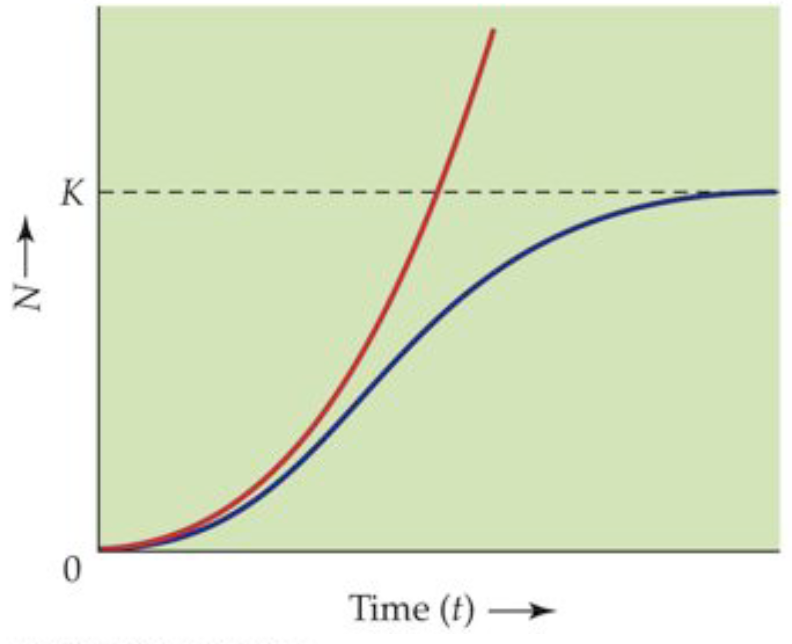
\includegraphics[width=.6 \textwidth]{./images_moores/Logistic_Exponential_Growth.png}
    \centering
    \caption{Visualization of exponential growth (red) and logistic growth (blue) \cite{cain2011ecology}.}
    \label{Logistic_Exponential_Growth}
\end{figure}


% %%%%%%%%%%%%%%%%%% Responsibility of Emissions %%%%%%%%%%%%%%%%%%%%%%%%%%
% \section{Appendix: Responsibility of Emissions}\label{SECTION_APPENDIX_RESPONSIBILITY_OF_EMISSIONS}
% The international community takes a production-based approach to measuring a country's emissions: a country is responsible for the emissions associated with the extraction of raw materials, production of goods and disposal of waste within their borders. This system forms the basis of the United Nations Framework Convention on Climate Change (UNFCCC) international carbon accounting systems and efforts to mitigate carbon emissions, including the Kyoto Protocol and the Paris Agreement \cite{unfccc2009kyoto, unfccc2015paris}. This accounting decision means a country's emission reduction commitments do not include emissions attributed to their imports---essentially, countries are allowed to export their emissions. This has coincided with a shift of energy intensive industries from developed to developing countries, which often are less energy efficient. For example, 23\% of China's total CO$_2$ emissions in 2004 came from its net exports (Figure \ref{emissions_China_export}) \cite{wang2007owns}.

% \begin{figure}[h]
%     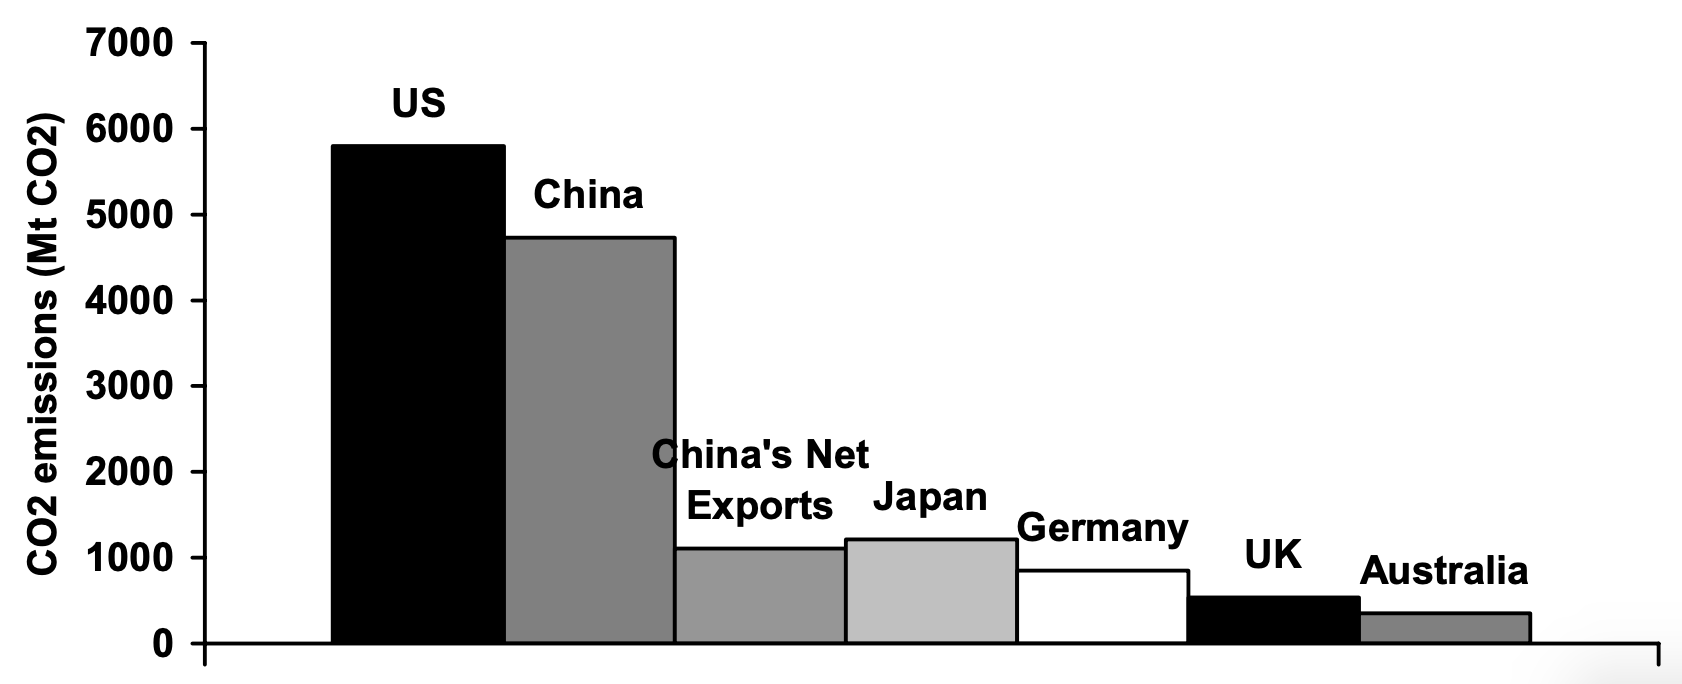
\includegraphics[width=.9 \textwidth]{./images/emissions_China_export.png}
%     \centering
%     \caption{CO$_2$ emissions from China's net exports in 2004 in comparison with selected national emissions figures \cite{wang2007owns}.}
%     \label{emissions_China_export}
% \end{figure}

% By measuring emissions based on production, rather than consumption, it raises the issues of equity: who is responsible for the emissions? Should responsibility for
% emissions be allocated to countries that \textit{produce} goods and services or to the countries that \textit{consume} the products and services? Critiques and potential improvements to this metric have been discussed \cite{tukker2020consumption, wang2007owns} and we recommend the reader to dive into them further if interested.

%%%%%%%%%%%%%%%%%%% Other Fantastic Quotes %%%%%%%%%%%%%%%%%%%%%%%%%%%%%
% “If you define the goal of a society as GNP, that society will do its best to produce GNP. It will not produce welfare, equity, justice, or efficiency unless you define a goal and regularly measure and report the state of welfare, equity, justice, or efficiency. The world would be a different place if instead of competing to have the highest per capita GNP, nations competed to have the highest per capita stocks of wealth with the lowest throughput, or the lowest infant mortality, or the greatest political freedom, or the cleanest environment, or the smallest gap between the rich and the poor.”
% ― Donella H. Meadows, Thinking in Systems: A Primer


% Homer Dixon, The Ingenuity Gap

\end{document}